%\chapter{Introduction}
%\label{Introduction1} 
%
%
%\section{Overview: Features and Setup}
%
%\subsection{Features}
%The mpFormulaPy distribution consists of two parts: the mpFormulaPy Library and the mpFormulaPy Toolbox.
%
%\subsection{The mpFormulaPy Library}
%The mpFormulaPy Library is a collection of numerical functions and procedures in multiprecision arithmetic. It is intended to be usable on multiple platforms (i.e. platforms supported by a recent version of Python) and is provided in the form of source code in Python. 
%
%The following numerical types are supported:
%
%\begin{itemize}		
%  \item The conventional double (64 bit) precision binary floating point type (double in C).
%  \item The mpf arbitray precision binary floating point type of the mpmath library.
%  \item The mpi arbitray precision interval arithmetic binary floating point type of the mpmath library.
%  \item The mpc arbitray precision complex binary floating point type of the mpmath library. 
%  \item The mpci arbitray precision complex interval arithmetic binary floating point type of the mpmath library.
%  \item The long arbitray precision integer type of the Python library. 
%  \item The Fraction arbitray precision rational type of the Python library. 
%  \item The Decimal arbitray precision decimal floating point type of the Python library. 
%\end{itemize}
%
%All of these types are available as real and complex scalars. vectors, and matrices.
%
%\vpara
%The mpFormulaPy Library is based on mpmath \cite{mpmath}, and the standard Python Library, including fractions.py and decimal.py.
%	
%\subsection{The mpFormulaPy Toolbox}	
%The mpFormulaPy Toolbox provides a setup with the Ironpython compiler 2.7.4 for the Windows platform with multiple interfaces:
%
%\begin{itemize}	
%\item A .NET Framework 4.0 interface: arithmetic functions, operators and procedures are accessible in a familiar syntax. Both 32 bit and 64 bit versions are provided. This interface makes the numerical routines available to all languages with .NET Framework support, including VB.NET, C\#, JScript 2010, F\#, MS C++ (CLI), IronPython and Matlab.
%\item A COM (Component Object Model) interface: multiprecision arithmetic functions and procedures, with arithmetic operators emulated as properties. Both 32 bit and 64 bit versions are provided. This interface makes the numerical routines available to all languages with COM support, including VBScript, JScript (Windows Script Host), Visual Basic for Applications, Visual Basic 6.0, OpenOffice  Basic, Lua, Ruby, PHP CLI, Perl, Python, R (Statistical System) and Mathematica.
%%\item A Java interface (Java SDK 1.7 or later): multiprecision arithmetic functions and procedures, with arithmetic operators emulated as properties. Both 32 bit and 64 bit versions are provided. Based on jni4net \citep{Savara2011}.
%%\item A SQLite interface: provides access from SQL to the numerical routines to manipulate arbitrary precisons numbers stored as strings.	Based on the System.Data.SQLite \citep{Hipp2014}.
%\item A Names Pipes and Command Line interface: this is designed to make sure that the calling application and the routines in the library are executed in separate processes, greatly enhancing stability. 
%
%\end{itemize}
%	
%In addition, the mpFormulaPy Toolbox offers the following features:	
%	
%\begin{itemize}		
%\item A compact IDE for VB.NET and C\# (no need to install Visual Studio). The IDE provides a Code Editor, Windows Forms Designer, Debugger, Profiler, Unit Tester and Microsoft Visual Studio compatible project files. Based on a trimmed version of Sharp Develop  \citep{SharpDevelop2013}.
%\item A Microsoft Excel (versions 2000 to 2013) interface: multiprecision arithmetic functions are provided for use in spreadsheet cells, using Excel's XLL interface. It is also possible to write user-defined functions and procedures in multiprecision arithmetic (provided as add-ins written in VB.NET or C\#), which run even if macro security is set to "disable all macros". Based on Excel-DNA \citep{vanDrimmelen2013}.	
%\item Full access for VB.NET and C\# to the object model of MS Excel (including Intellisense support in the Code Editor). All Microsoft Excel versions from 2000 to 2013,  both 32 bit and 64 bit (only 2010 and 2013), are supported, and no other software (like PIAs) is needed. Based on NetOffice \citep{Lange2013}.
%\item An OpenOffice Calc (versions 2.1 or later, incl. Apache OpenOffice Calc or LibreOffice Calc) interface: multiprecision arithmetic functions are provided for use in spreadsheet cells, using the OpenOffice Basic interface. It is also possible to write user-defined functions and procedures in multiprecision arithmetic (provided as add-ins written in VB.NET or C\#).	
%\end{itemize}
%
%
%
%
%\subsection{System Requirement}
%\label{System Requirements}
%This mpFormulaPy Toolbox has the following system requirement:
%
%\begin{itemize}
%  \item Microsoft Windows with Microsoft .NET Framework version 4.x (Full).
%\end{itemize}
%
%
%This mpFormulaPy Toolbox can take advantage of the following software:
%
%\begin{itemize}
%  \item Adobe Reader 8 or later, for use with mpFormulaPy's interactive help-system.
%  \item Microsoft Office 2000 or later.
%  \item OpenOffice (versions 2.1 or later), or Apache OpenOffice or LibreOffice.
%\end{itemize}
%
%
%\subsection{Installation}
%\label{Installation}
%The mpFormulaPy Library and Toolbox can be downloaded from 
%
%\vpara
%\href{http://mpFormula.github.io/Py/}{http://mpFormula.github.io/Py/}. 
%
%\vpara
%Unzip the downloaded file in a directory for which you have write-access.
%
%
%
%
%
%\section{License}
%\label{mpFormulaLicense}
%
%The mpFormulaPy Library and Toolbox is free software. It is licensed under the GNU Lesser General Public License (LGPL), Version 3 (see appendix \ref{LGPLv3}).
%The manual for the mpFormulaPy Toolbox (this document) is licensed under the GNU Free Documentation License, Version 1.3 (see appendix \ref{GNUFDL}).
%
%
%
%
%\section{No Warranty}
%\label{No Warranty} 
%
%There is no warranty. See the GNU  Lesser General Public License, Version 3 (see appendix \ref{LGPLv3}) for details.
%
%
%\section{Related Software}
%
%The mpFormulaC  Library and Toolbox provides fast multiprecision routines written in C, with interfaces to CPython, R, .NET and COM. It can be downloaded from 
%
%\href{http://mpFormula.github.io/C/}{http://mpFormula.github.io/C/}. 
%
%



\chapter{Introduction}
\label{Introduction1} 



\section{Overview: Features and Setup}


\subsection{Features}
The mpFormulaC distribution consists of two parts: the mpFormulaC Library and the mpFormulaC Toolbox.

\subsection{The mpFormulaC Library}

The mpFormulaC Library is a collection of numerical functions and procedures in multiprecision arithmetic. It is intended to be usable on multiple platforms (i.e. platforms supported by a recent version of the GNU Compiler Collection, e.g. Windows, GNU/Linux, Mac OS) and is provided in the form of source code, with interfaces to C and C++. 

The following multi-precision types are supported:

\begin{itemize}		
	\item The FMPZ arbitrary precision integer type of the FLINT library. 
	\item The FMPQ arbitrary precision rational type of the FLINT library. 
	\item The MPD arbitrary precision decimal floating point type of the libmpdec library. 
	\item The MPFR arbitrary precision real binary floating point type of the MPFR library.
	\item The MPC arbitrary precision complex binary floating point type of the MPC library.
	\item The ARB arbitrary precision real binary interval arithmetic floating point type of the ARB library.
	\item The ACB arbitrary precision complex binary interval arithmetic floating point type of the ARB library.   
\end{itemize}

In addition, the following hardware-based floating-point types are supported:

\begin{itemize}		
	\item The conventional single (32 bit) precision real binary floating point type (float in C).
	\item The conventional single (32 bit) precision complex binary floating point type (float in C).	
	\item The conventional double (64 bit) precision real binary floating point type (double in C).
	\item The conventional double (64 bit) precision complex binary floating point type (double in C).	
	\item The extended precision (80 bit) real binary floating point type of the Intel FPU.
	\item The extended precision (80 bit) complex binary floating point type of the Intel FPU.	
\end{itemize}


All of these types are available as scalars, vectors, and matrices.

\vpara
The mpFormulaC Library is based on GMP \citep{Granlund12}, MPFR \citep{MPFR_2007}, MPC \citep{mpc_2012}, MPFRC++ \citep{Holoborodko2012}, gmpfrxx \citep{Wilkening2008}, libmpdec \citep{mpd_2012}, Eigen \citep{Guennebaud2010}, Boost Math \citep{boost_math}, Boost Random \citep{boost_random}, FLINT \cite{Hart2010}, ARB \cite{arb}.



\subsection{The mpFormulaC Toolbox}	
The mpFormulaC Toolbox provides precompiled binaries for the Windows platform with multiple interfaces:

\begin{itemize}	
	
	\item A C interface: provides the most direct and efficient access to the numerical routines, and can be used as basis for other interfaces. Is intended to work with most C compilers, and can also be used from Objective C.
	\item A C++ interface: provides a rich set of multiprecision arithmetic functions, operators and procedures, which are accessible in a familiar syntax, thanks to operator overloading. Both 32 bit and 64 bit versions are provided. Is intended to work with most C++ compilers, and can also be used from Objective C++.
	\item A COM (Component Object Model) interface: multiprecision arithmetic functions and procedures, with arithmetic operators emulated as properties. Both 32 bit and 64 bit versions are provided. This interface makes the numerical routines available to all languages with COM support, including VBScript, JScript (Windows Script Host), Visual Basic for Applications, Visual Basic 6.0, OpenOffice  Basic, Lua, Ruby, PHP CLI, Perl, Python, R (Statistical System) and Mathematica.
	\item A .NET Framework 4.0 interface: As for C++, arithmetic functions, operators and procedures are accessible in a familiar syntax. Both 32 bit and 64 bit versions are provided. This interface makes the numerical routines available to all languages with .NET Framework support, including VB.NET, C\#, JScript 2010, F\#, MS C++ (CLI), IronPython and Matlab.
	%\item A Java interface (Java SDK 1.5 or later): multiprecision arithmetic functions and procedures, with arithmetic operators emulated as properties. Both 32 bit and 64 bit versions are provided. Based on jni4net \citep{Savara2011}.
	%\item A SQLite interface: provides access from SQL to the numerical routines to manipulate arbitrary precisons numbers stored as strings.	Based on the System.Data.SQLite \citep{Hipp2014}.
	\item A Names Pipes and Command Line interface: this is designed to make sure that the calling application and the routines in the library are executed in separate processes, greatly enhancing stability. 
	
\end{itemize}




\subsection{System Requirement}
\label{System Requirements}
This mpFormulaC Library and Toolbox has the following system requirement:

\begin{itemize}
	\item Microsoft Windows with Microsoft .NET Framework version 4.x (Full).
\end{itemize}



\subsection{Installation}
\label{Installation}
The mpFormulaC Library and Toolbox can be downloaded from 

\vpara
\href{http://mpFormula.github.io/C/}{http://mpFormula.github.io/C/}. 

\vpara
Unzip the downloaded file in a directory for which you have write-access.




\section{License}
\label{mpFormulaLicense}

The mpFormulaC Library and Toolbox is free software. It is overall licensed under the GNU General Public License, Version 3 (see appendix \ref{GPLv3}). Note however that the underlying libraries come with their own license terms; see the appendix for details.

The manual for the mpFormulaC Library and Toolbox (this document) is licensed under the GNU Free Documentation License, Version 1.3 (see appendix \ref{GNUFDL}).




\section{No Warranty}
\label{No Warranty} 

There is no warranty. See the GNU General Public License, Version 3 (see appendix \ref{GPLv3}) for details.


\section{Related Software}

The mpFormulaPy Library and Toolbox provides multiprecision routines written in Python, with interfaces to CPython, R, .NET and COM. It can be downloaded from 

\href{http://mpFormula.github.io/Py/}{http://mpFormula.github.io/Py/}. 





\chapter{Tutorials}
\label{Tutorials} 

\section{Why multi-precision arithmetic?}
\label{Why multiprecision arithmetic}

An introduction to the problems of rounding errors and catastrophic cancellation can be found in \cite{Goldberg91whatevery}. Excellent reference texts are  \cite{Higham2002} and \cite{Higham2009}.

In the following paragraphs we will give a few examples of how widely used programs like MS Excel or Libreoffice Calc can give wrong results due to the fact that they are using double precision arithmetic and not multi-precision arithmetic

\subsection{Example 1: Sums}

Sums are often calculated exactly if all summands have an exact representation. If this is not the case, results can be unpredictable. In MS Excel, the formula

\begin{verbatim}
=SUM(10000000000,-16000000000,6000000000)
\end{verbatim}
 will give the correct result  \verb|0|, but the analogous formula
 \begin{verbatim}
=SUM(1E+40,-1.6E+40,6E+39)
 \end{verbatim}
returns \verb|1.20893E+24| instead of the correct result \verb|0|.

\subsection{Example 2: Standard Deviation}
Like sums, variances and standard deviations are often calculated exactly if all arguments have an exact representation. If this is not the case, results can again be unpredictable. In MS Excel, the formula
 \begin{verbatim}
=VAR(1E+30,1E+30,1E+30)
 \end{verbatim}
returns \verb|2.97106E+28| instead of the correct result \verb|0|, which should be the obvious results since all arguments are the same.


\subsection{Example 3: Overflow and underflow}

In many situations where the final result is representable in double precision, some of the interim results cause overflow or underflow. A popular example is the function $f(x,y) = \sqrt{x^2+y^2}$. With $x=3 \cdot 10^{300}$ and $y=4 \cdot 10^{300}$ the result $f(x,y) = 5 \cdot 10^{300}$ is representable in double precision, but the (naive) calculation will overflow.



\subsection{Example 4: Polynomials}

Consider the following example \cite{Cuyt_2001}: 

\vpara
For $a=77617$ and $b=33096$, calculate

\begin{equation}
Y = 333.75 b^6 + a^2  (11 a^2  b^2 - b^6 - 121 b^4 - 2) + 5.5  b^8 + \frac{a}{2b} 
\end{equation}

The correct result is $Y = -54767 / 66192 = -0.827396...$




\subsection{Example 5: Trigonometric Functions}

Trigonometric functions are sensitive to small perturbations. 

\vpara
In double precision and binary floating point arithmetic, the tangent of $x = 1.57079632679489$ is calculated as $\tan(x) = 1.48752 \cdot 10^{14}$, whereas the correct result is $\tan(x) = 1.51075 \cdot 10^{14}$. This amounts to an absolute error of $2.32287  \cdot 10^{12}$ and a relative error of $1.54\%$.

\vpara
There are also limits on the range of arguments, e.g. $\sin(10^{8})$ returns the value $0.931639...$ (with an relative error of $-6.22776 \cdot 10^{-13}$), whereas  $\sin(10^{9})$ returns an invalid result (the exact result is 0.545843...)





\subsection{Example 6: Logarithms and Exponential Functions}


Consider the following example \citep{Ghazi2010} : 

Determine 10 decimal digits of the constant

\begin{equation}
Y = 173746a + 94228b - 78487c, \quad \text{where } 
\end{equation}
\begin{equation}
a = \sin(10^{22}), b = \ln(17.1), c = \exp(0.42). 
\end{equation}

The expected result is $Y = -1.341818958 \cdot 10^{-12}$.





\subsection{Example 7: Linear Algebra}


\subsubsection{Linear Solver}
The following example is from \cite{Hofschuster2004}:

We want to solve the (ill-conditioned) system of linear equations $Ax = b$ with

\begin{equation}
A = \begin{pmatrix}
a_{11} & a_{12} \\
a_{21} & a_{22} 
\end{pmatrix}  = \begin{pmatrix}
64919121 & -159018721 \\
41869520.5 & -102558961 
\end{pmatrix}, b = \begin{pmatrix}
b_{1} \\
b_{2} 
\end{pmatrix}
= \begin{pmatrix}
1 \\
0
\end{pmatrix} , x = \begin{pmatrix}
x_{1} \\
x_{2} 
\end{pmatrix}
\end{equation}

The correct solution is $x_1 = 205117922$, $x_2 = 83739041$.

To solve this $2 \times 2$ system numerically we first use the well known formulas

\begin{equation}
x_1 = \frac{a_{22}}{a_{11}a_{22} - a_{12}a_{21}}, \quad x_2 = \frac{-a_{21}}{a_{11}a_{22} - a_{12}a_{21}},
\end{equation}

Calculating this directly in double precision gives the following wrong result:  

$x_1 = 102558961$, $x_2 = 41869520.5$

%Linear equation
%
%See also \cite{Hofschuster2001}.





\newpage
\section{Graphics using Latex}
\label{Tutorial: GraphicsLatex}


pgfplots \citep{Feuersanger_2014} - A TeX package to draw normal and/or logarithmic plots directly in TeX in two and three dimensions with a user-friendly interface and pgfplotstable - a TeX package to round and format numerical tables. Examples in manuals and/or on web site.

\vpara
\href{http://pgfplots.net/}{http://pgfplots.net/}. 


\vpara
\href{http://pgfplots.sourceforge.net/}{http://pgfplots.sourceforge.net/}. 

\vpara
\href{http://pgfplots.sourceforge.net/gallery.html}{http://pgfplots.sourceforge.net/gallery.html}. 

\vpara
\href{https://www.sharelatex.com/learn/Pgfplots\_package}{https://www.sharelatex.com/learn/Pgfplots\_package}. 



\begin{figure}[ht]
	\centering
	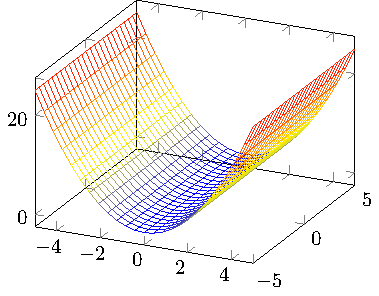
\includegraphics{figures/3Dplot.pdf}
	\caption{A pdf plot}
	\label{Fig pdf of the Distribution of the Sample Correlation Coefficient}
\end{figure}



\newpage
\section{Graphics using .NET Framework}
\label{Tutorial: Graphics}
The mpformulaPy toolbox offers a facility for producing 3D charts. The following pages give a few examples.

\begin{figure}[ht]
	\centering
	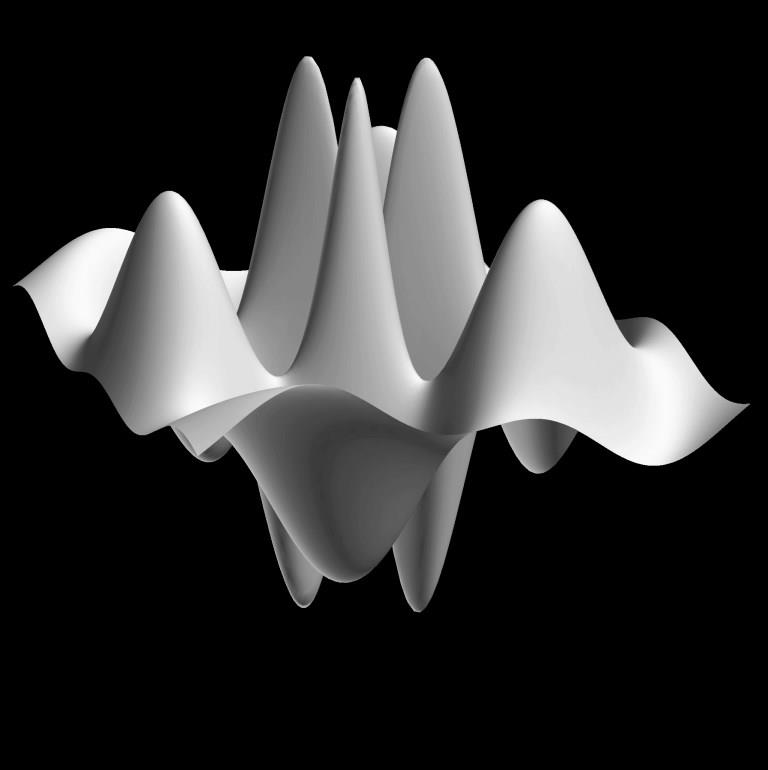
\includegraphics[scale=3.0]{Charts/jpg/SurfaceBlackAndWhite.jpg}
	\caption{plot of a 2-dimensional function}
	\label{Fig plot of a 2-dimensional function}
\end{figure}


The corresponding code is:
\lstset{language={[Sharp]C}}
\begin{lstlisting}
const double two_pi = 2 * Math.PI;
double r2 = x * x + z * z;
double r = Math.Sqrt(r2);
double theta = Math.Atan2(z, x);
result = Math.Exp(-r2) * Math.Sin(two_pi * r) * Math.Cos(3 * theta);
\end{lstlisting}


\newpage
\subsection{Surface plots for bivariate real functions}

The bivariate normal distribution has the following density:
\begin{equation}
	g(x,y;\rho) = \frac{1}{2 \pi \sqrt{1-\rho^2}} e^{\frac{-(x^2 -2\rho x y + y^2)}{2(1-\rho^2)}}
\end{equation}


\begin{figure}[ht]
	\centering
	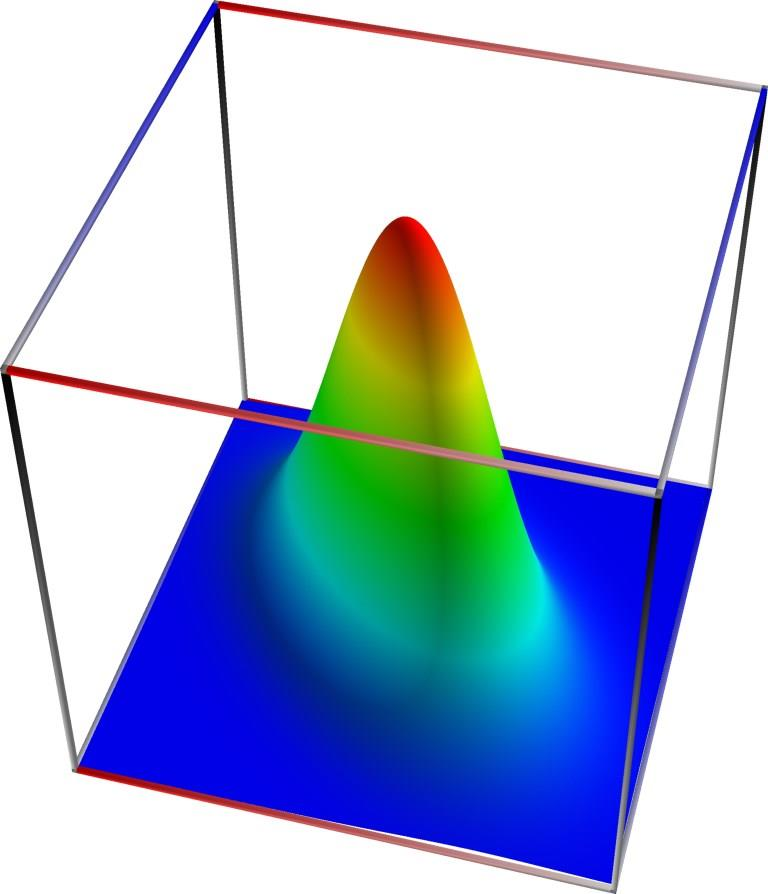
\includegraphics[scale=3.0]{Charts/jpg/BivariateNormal2.jpg}
	\caption{Surface plot of the probability density function of the bivariate normal distribution with $\rho = - 0.5$ }
	\label{Fig plot of the bivariate normal distribution}
\end{figure}


The corresponding code is:
\lstset{language={[Sharp]C}}
\begin{lstlisting}
const double two_pi = 2 * Math.PI;
double rho = -0.5;
double r2 = 1.0 - rho*rho;
double f = 1 / (two_pi * Math.Sqrt(r2));
double e = -(x*x - 2*rho*x*z + z*z)/(2*r2);
result = f * Math.Exp(e);
\end{lstlisting}


\newpage
\subsection{3D Plots of parametric functions}

\subsubsection{3D Plot of a Seashell}

This is a plot of a seashell. 

\begin{figure}[ht]
	\centering
	\includegraphics[scale=3.0]{Charts/jpg/Seashell.jpg}
	\caption[3D plot of a parametric function: Seashell]{3D plot of a parametric function: Seashell. umin = 0; umax = 6*Math.PI; umin = 0; umax = 6*Math.PI. Camera angles are $\theta = 135\degree$ and $\phi = -12\degree$.}
	\label{Fig 3D plot of a parametric function: Seashell}
\end{figure}


The parametrization is:
\lstset{language={[Sharp]C}}
\begin{lstlisting}
double a = Math.Exp(u / (6.0 * Math.PI));
double b = Math.Cos(v / 2.0);

x = 2.0 * (1.0 - a) * Math.Cos(u) * b * b;
z = 2.0 * (-1.0 + a) * Math.Sin(u) * b * b;
y = 1.0 - a * a - Math.Sin(v) * (1.0 - a);
\end{lstlisting}



\newpage
\subsubsection{3D Plot of Kuen's surface}

This is a plot of Kuen's surface. 

\begin{figure}[ht]
	\centering
	
\includegraphics[scale=3.0]{Charts/jpg/KuenSurface.jpg}
	\caption[3D plot of Kuen's surface]{3D plot of a parametric function: Kuen's surface. umin = -4.5; umax = 4.5; vmin = 0.01; vmax = 3.14. Camera angles are $\theta = 135\degree$ and $\phi = -12\degree$.}
	\label{Fig 3D plot of a parametric function: Kuen's surface}
\end{figure}


The parametrization is:
\lstset{language={[Sharp]C}}
\begin{lstlisting}
double a = 1.0 * Math.Sin(v);
double b = 1.0 + u * u * a * a;

x = 2.0 * a * (Math.Cos(u) + u * Math.Sin(u)) / b;
z = 2.0 * a * (Math.Sin(u) - u * Math.Cos(u)) / b;
y = Math.Log(Math.Tan(v/2.0)) + 2.0 * Math.Cos(v) / b;
\end{lstlisting}



\newpage
\subsubsection{3D Plot of Klein's Bottle}

This is a plot of Klein's Bottle. 

\begin{figure}[ht]
	\centering
	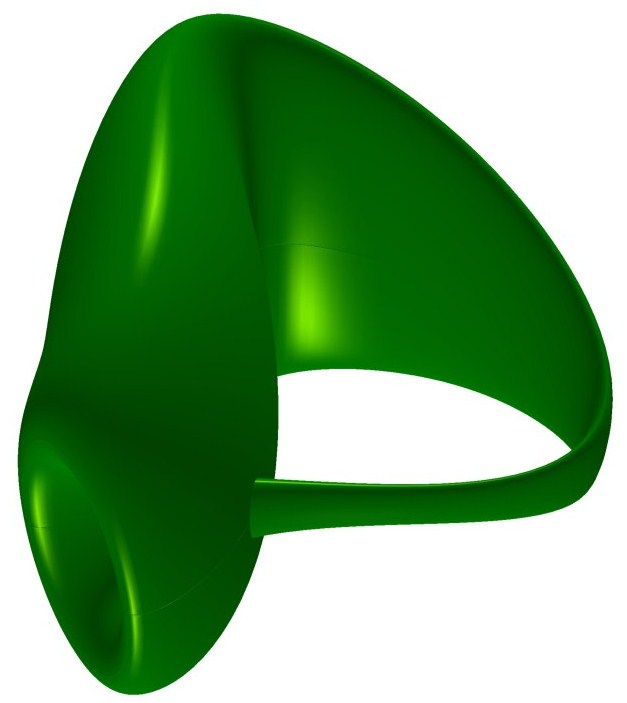
\includegraphics[scale=3.0]{Charts/jpg/KleinBottle.jpg}
	\caption[3D plot of Klein's Bottle]{3D plot of a parametric function: Klein's Bottle. umin = 0.0; umax = 3.14; vmin = 0.0; vmax = 6.28. Camera angles are $\theta = 135\degree$ and $\phi = -12\degree$.}
	\label{Fig 3D plot of a parametric function: Klein's Bottle}
\end{figure}


The following parametrization is due to Robert Israel (with some rearrangements):
\lstset{language={[Sharp]C}}
\begin{lstlisting}
double a = Math.Cos(u);
double b = Math.Sin(u);
double c = Math.Cos(v);
double a2 = a * a;
double a4 = a2 * a2;

x = -(2.0/15.0) * a * (3*c + b*(-30 + a4*(90 - 60*a2) + 5*a*c));
z = -(1.0/15.0) * b*b * (c*b* (3 - 48*a4  + 5*a*b*(1 - 16*a4)) - 60);
y = (2.0/15.0) * (3 + 5*a*b) * Math.Sin(v);
\end{lstlisting}





\newpage
\subsection{Surface plots of complex functions}
\label{Graphics: Surface plots of complex functions}
It is straight forward to produce surface plots of complex functions; these are available in two forms:

\vpara
As plots of the real and imaginary component:

\begin{figure}[ht]
	\centering
	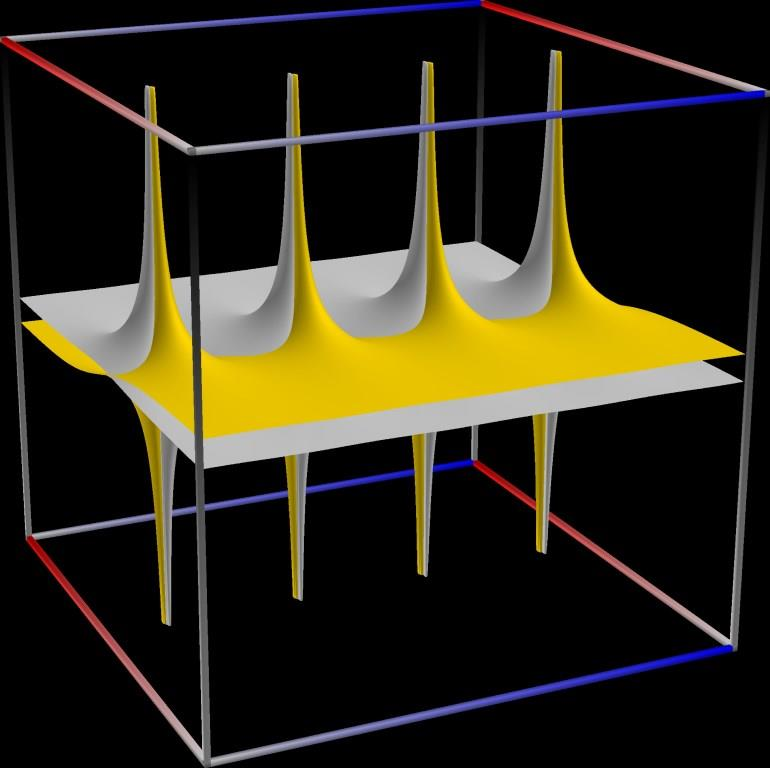
\includegraphics[scale=3.0]{Charts/jpg/ComplexSurfacePlotRealAndImaginary.jpg}
	\caption[Surface plot of the real and imaginary component of $z = \tan(x + iy)$]{Surface plot of the real ("silver") and imaginary ("gold") component of $z = \tan(x + iy)$, $-3 \leq x \leq 3$ (blue axis), $-2 \pi \leq y \leq 2\pi$ (red axis), $-10 \leq z \leq 10$ (black axis). $z$ values are truncated at $\pm 10$. There is a branch cut along the negative real axis. Camera angles are $\theta = 135\degree$ and $\phi = -12\degree$.}
	\label{Fig plot of the re and im of complex tangent}
\end{figure}



%\subsection{Pretty Formatting (specify extra digits)}

\newpage
%\subsection{File Output}
As plots of the absolute value with the phase color-coded:


\begin{figure}[ht]
	\centering
	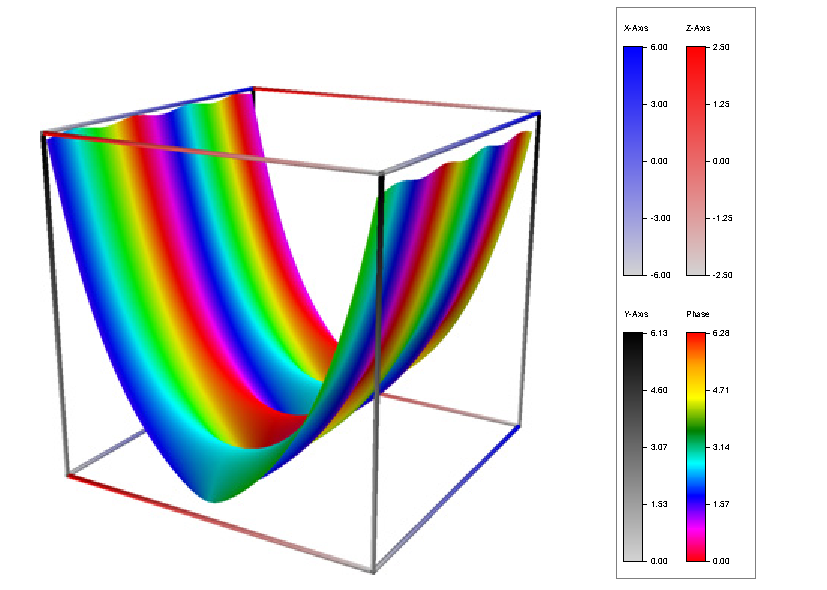
\includegraphics[scale=1.2]{Charts/pdf/SurfacePlotWithScales.pdf}
	\caption[Surface plot of the magnitude of $z = \sin(x + iy)$]{Surface plot of the magnitude and phase (color-coded) of $z = \sin(x + iy)$, $-3 \leq x \leq 3$ (blue axis), $-2 \pi \leq y \leq 2\pi$ (red axis), $-10 \leq z \leq 10$ (black axis). $z$ values are truncated at $\pm 10$. There is a branch cut along the negative real axis. Camera angles are $\theta = 135\degree$ and $\phi = -12\degree$. } 
	\label{Fig plot of the magnitude of complex sine}
\end{figure}




%
%
%\newpage
%\section{Eval, Options, Tables and Charts}
%
%The following functions provide quick access to function evaluations and charts:
%
%\vspace{0.3cm}
%\begin{mpFunctionsExtract}
%	\mpFunctionOne
%	{Eval? String?  the result of the evaluation of an arithmetic expression, containing number and functions, but no variables.}
%	{Expression? String? an arithmetic expression.}
%\end{mpFunctionsExtract}
%
%
%\vspace{0.3cm}
%\begin{mpFunctionsExtract}
%	\mpFunctionOne
%	{Options? String?  an identifier for a set of calculation options.}
%	{BaseOptions? String? an identifier for a set of base calculation options.}
%\end{mpFunctionsExtract}
%
%
%\vspace{0.3cm}
%\begin{mpFunctionsExtract}
%	\mpFunctionOne
%	{Table? Range?  an identifier for a set of calculation options.}
%	{TableRef? String? a reference for a table.}
%\end{mpFunctionsExtract}
%
%
%\vspace{0.3cm}
%\begin{mpFunctionsExtract}
%	\mpFunctionOne
%	{Chart? String?  an identifier for an XML Chart.}
%	{Data? Range? a reference for a data table.}
%\end{mpFunctionsExtract}
%
%


\chapter{Python: Built-in numerical types}


The following sections describe the standard types that are built into the interpreter.

The principal built-in types are numerics, sequences, mappings, classes, instances and exceptions.

Some collection classes are mutable. The methods that add, subtract, or rearrange their members in place, and do not return a specific item, never return the collection instance itself but None.

Some operations are supported by several object types; in particular, practically all objects can be compared, tested for truth value, and converted to a string (with the repr() function or the slightly different str() function). The latter function is implicitly used when an object is written by the print() function.

\section{Truth Value Testing}

Any object can be tested for truth value, for use in an if or while condition or as operand of the Boolean operations below. The following values are considered false:

\vpara
None

False

zero of any numeric type, for example, \verb| 0, 0.0, 0j|.

any empty sequence, for example, \verb| '', (), []|.

any empty mapping, for example, \verb| {}|.

instances of user-defined classes, if the class defines a \_\_bool\_\_() or \_\_len\_\_() method, when that method returns the integer zero or bool value False.

\vpara
All other values are considered true $-$ so objects of many types are always true.

Operations and built-in functions that have a Boolean result always return 0 or False for false and 1 or True for true, unless otherwise stated. (Important exception: the Boolean operations or and and always return one of their operands.)

\section{Boolean Operations:  and, or, not}

These are the Boolean operations, ordered by ascending priority:



\begin{table}[ht]
	\centering
	\begin{tabular}{|l|l|l|}
		\hline
		Operation & Result & Notes\\
		\hline
		\verb|x or y| & if x is false, then y, else x &  (1) \\
		\verb|x and y| & if x is false, then x, else y & (2)  \\
		\verb|not x| & if x is false, then True, else False & (3)  \\								
		\hline
	\end{tabular}
	%	\caption{\result}
	%	\label{\result} 
\end{table}


  

Notes:
1.This is a short-circuit operator, so it only evaluates the second argument if the first one is False.
2.This is a short-circuit operator, so it only evaluates the second argument if the first one is True.
3.not has a lower priority than non-Boolean operators, so not a == b is interpreted as not (a == b), and a == not b is a syntax error.

\section{Comparisons}

There are eight comparison operations in Python. They all have the same priority (which is higher than that of the Boolean operations). Comparisons can be chained arbitrarily; for example, x < y <= z is equivalent to x < y and y <= z, except that y is evaluated only once (but in both cases z is not evaluated at all when x < y is found to be false).

This table summarizes the comparison operations:


\begin{table}[ht]
	\centering
	\begin{tabular}{|l|l|}
		\hline
		Operation & Meaning \\
		\hline
		\verb|<| & strictly less than \\
		\verb|<=| & less than or equal  \\							
		\verb|>| & strictly greater than \\
		\verb|>=| & greater than or equal  \\							
		\verb|==| & equal \\
		\verb|!=| & not equal  \\							
		\verb|is| & object identity \\
		\verb|is not| & negated object identity  \\							
		\hline
	\end{tabular}
	%	\caption{\result}
	%	\label{\result} 
\end{table}


Objects of different types, except different numeric types, never compare equal. Furthermore, some types (for example, function objects) support only a degenerate notion of comparison where any two objects of that type are unequal. The <, <=, > and >= operators will raise a TypeError exception when comparing a complex number with another built-in numeric type, when the objects are of different types that cannot be compared, or in other cases where there is no defined ordering.

Non-identical instances of a class normally compare as non-equal unless the class defines the \_\_eq\_\_() method.

Instances of a class cannot be ordered with respect to other instances of the same class, or other types of object, unless the class defines enough of the methods \_\_lt\_\_(), \_\_le\_\_(), \_\_gt\_\_(), and \_\_ge\_\_() (in general, \_\_lt\_\_() and \_\_eq\_\_() are sufficient, if you want the conventional meanings of the comparison operators).

The behavior of the is and is not operators cannot be customized; also they can be applied to any two objects and never raise an exception.

Two more operations with the same syntactic priority, in and not in, are supported only by sequence types (below).


\section{Numeric Types - int, float, complex}

There are three distinct numeric types: integers, floating point numbers, and complex numbers. In addition, Booleans are a subtype of integers. Integers have unlimited precision. Floating point numbers are usually implemented using double in C; information about the precision and internal representation of floating point numbers for the machine on which your program is running is available in sys.float\_info. Complex numbers have a real and imaginary part, which are each a floating point number. To extract these parts from a complex number z, use z.real and z.imag. (The standard library includes additional numeric types, fractions that hold rationals, and decimal that hold floating-point numbers with user-definable precision.)

\vpara
Numbers are created by numeric literals or as the result of built-in functions and operators. Unadorned integer literals (including hex, octal and binary numbers) yield integers. Numeric literals containing a decimal point or an exponent sign yield floating point numbers. Appending 'j' or 'J' to a numeric literal yields an imaginary number (a complex number with a zero real part) which you can add to an integer or float to get a complex number with real and imaginary parts.

\vpara
Python fully supports mixed arithmetic: when a binary arithmetic operator has operands of different numeric types, the operand with the "narrower" type is widened to that of the other, where integer is narrower than floating point, which is narrower than complex. Comparisons between numbers of mixed type use the same rule. [2] The constructors int(), float(), and complex() can be used to produce numbers of a specific type.

\vpara
All numeric types (except complex) support the following operations, sorted by ascending priority (operations in the same box have the same priority; all numeric operations have a higher priority than comparison operations):


\begin{table}[ht]
	\centering
	\begin{tabular}{|l|l|l|}
		\hline
		Operation & Result & Notes\\
		\hline
		x + y & sum of x and y &   \\
		x - y & difference of x and y &   \\
		x * y & product of x and y &   \\				
		x / y & quotient of x and y &  (1) \\
		x // y & floored quotient of x and y &  \\
		x \% y & remainder of x / y &  (2) \\				
		-x & x negated &   \\
		+x & x unchanged &   \\
		abs(x) & absolute value or magnitude of x &   \\
		int(x) & x converted to integer &  (3)(6) \\
		float(x) & x converted to floating point &  (4)(6) \\
		complex(re, im) & a complex number with real part re, imaginary part im. &  \\
		 & im defaults to zero. &  (6) \\
		c.conjugate() & conjugate of the complex number c &  No \\
		divmod(x, y) & the pair (x // y, x \% y) &  (2) \\
		pow(x, y)  & x to the power y &  (5) \\
		x ** y &  x to the power y &  (5) \\
		math.trunc(x) &  x truncated to Integral &  (7) \\
		round(x[, n]) &  x rounded to n digits, rounding half to even. & \\
		 & If n is omitted, it defaults to 0. &  (7) \\
		math.floor(x) &  the greatest integral float $\le$ x &  (7) \\
		math.ceil(x) &  the least integral float $\ge$ x &  (7) \\
		\hline
	\end{tabular}
	%	\caption{\result}
	%	\label{\result} 
\end{table}
    


Notes:

1.Also referred to as integer division. The resultant value is a whole integer, though the result's type is not necessarily int. The result is always rounded towards minus infinity: 1//2 is 0, (-1)//2 is -1, 1//(-2) is -1, and (-1)//(-2) is 0.

\vpara
2.Not for complex numbers. Instead convert to floats using abs() if appropriate.

\vpara
3.Conversion from floating point to integer may round or truncate as in C; see functions math.floor() and math.ceil() for well-defined conversions.

\vpara
4.float also accepts the strings "nan" and "inf" with an optional prefix "+" or "-" for Not a Number (NaN) and positive or negative infinity.

\vpara
5.Python defines pow(0, 0) and 0 ** 0 to be 1, as is common for programming languages.

\vpara
6.The numeric literals accepted include the digits 0 to 9 or any Unicode equivalent (code points with the Nd property).

7.Only real types (int and float).

See http://www.unicode.org/Public/6.0.0/ucd/extracted/DerivedNumericType.txt for a complete list of code points with the Nd property.


For additional numeric operations see the math and cmath modules.

\section{Long integers}

\subsection{Bitwise Operations on Integer Types}

Bitwise operations only make sense for integers. Negative numbers are treated as their 2’s complement value (this assumes a sufficiently large number of bits that no overflow occurs during the operation).

The priorities of the binary bitwise operations are all lower than the numeric operations and higher than the comparisons; the unary operation ~ has the same priority as the other unary numeric operations (+ and -).

This table lists the bitwise operations sorted in ascending priority (operations in the same box have the same priority):



\begin{table}[ht]
	\centering
	\begin{tabular}{|l|l|l|}
		\hline
		Operation & Result & Notes\\
		\hline
		\verb!x | y! & bitwise or of x and y &   \\
		\verb|x ^ y| & bitwise exclusive or of x and y &   \\
		\verb|x & y| & bitwise and of x and y &   \\				
		\verb|x << n| & x shifted left by n bits & (1)(2) \\
		\verb|x >> n| & x shifted right by n bits & (1)(3) \\
		\verb|~x| & the bits of x inverted &  \\				
		\hline
	\end{tabular}
	%	\caption{\result}
	%	\label{\result} 
\end{table}

    

Notes:
1.Negative shift counts are illegal and cause a ValueError to be raised.
2.A left shift by n bits is equivalent to multiplication by pow(2, n) without overflow check.
3.A right shift by n bits is equivalent to division by pow(2, n) without overflow check.

\subsection{Additional Methods on Integer Types}
 
The int type implements the numbers.Integral abstract base class. In addition, it provides one more method:

\subsubsection{int.bit\_length()}

Return the number of bits necessary to represent an integer in binary, excluding the sign and leading zeros:

\lstset{language={Python}}
\begin{lstlisting}
>>>>>> n = -37
>>> bin(n)
'-0b100101'
>>> n.bit_length()
6
\end{lstlisting}

More precisely, if x is nonzero, then x.bit\_length() is the unique positive integer k such that 2**(k-1) <= abs(x) < 2**k. Equivalently, when abs(x) is small enough to have a correctly rounded logarithm, then k = 1 + int(log(abs(x), 2)). If x is zero, then x.bit\_length() returns 0.

Equivalent to:

\lstset{language={Python}}
\begin{lstlisting}
def bit_length(self):
s = bin(self)       # binary representation:  bin(-37) --> '-0b100101'
s = s.lstrip('-0b') # remove leading zeros and minus sign
return len(s)       # len('100101') --> 6
\end{lstlisting}


\subsubsection{int.to\_bytes}
New in version 3.1.

int.to\_bytes(length, byteorder, *, signed=False)
Return an array of bytes representing an integer.

\lstset{language={Python}}
\begin{lstlisting}
>>>>>> (1024).to_bytes(2, byteorder='big')
b'\x04\x00'
>>> (1024).to_bytes(10, byteorder='big')
b'\x00\x00\x00\x00\x00\x00\x00\x00\x04\x00'
>>> (-1024).to_bytes(10, byteorder='big', signed=True)
b'\xff\xff\xff\xff\xff\xff\xff\xff\xfc\x00'
>>> x = 1000
>>> x.to_bytes((x.bit_length() // 8) + 1, byteorder='little')
b'\xe8\x03'
\end{lstlisting}

The integer is represented using length bytes. An OverflowError is raised if the integer is not representable with the given number of bytes.

The byteorder argument determines the byte order used to represent the integer. If byteorder is "big", the most significant byte is at the beginning of the byte array. If byteorder is "little", the most significant byte is at the end of the byte array. To request the native byte order of the host system, use sys.byteorder as the byte order value.

The signed argument determines whether two’s complement is used to represent the integer. If signed is False and a negative integer is given, an OverflowError is raised. The default value for signed is False.

\subsubsection{int.from\_bytes}
New in version 3.2.

classmethod int.from\_bytes(bytes, byteorder, *, signed=False)
Return the integer represented by the given array of bytes.

\lstset{language={Python}}
\begin{lstlisting}
>>>>>> int.from_bytes(b'\x00\x10', byteorder='big')
16
>>> int.from_bytes(b'\x00\x10', byteorder='little')
4096
>>> int.from_bytes(b'\xfc\x00', byteorder='big', signed=True)
-1024
>>> int.from_bytes(b'\xfc\x00', byteorder='big', signed=False)
64512
>>> int.from_bytes([255, 0, 0], byteorder='big')
16711680
\end{lstlisting}

The argument bytes must either be a bytes-like object or an iterable producing bytes.

The byteorder argument determines the byte order used to represent the integer. If byteorder is "big", the most significant byte is at the beginning of the byte array. If byteorder is "little", the most significant byte is at the end of the byte array. To request the native byte order of the host system, use sys.byteorder as the byte order value.

The signed argument indicates whether two’s complement is used to represent the integer.


\subsection{Additional Methods on Float}

The float type implements the numbers.Real abstract base class. float also has the following additional methods.

\subsubsection{float.as\_integer\_ratio()}

Return a pair of integers whose ratio is exactly equal to the original float and with a positive denominator. Raises OverflowError on infinities and a ValueError on NaNs.

\subsubsection{float.is\_integer()}

Return True if the float instance is finite with integral value, and False otherwise:

\lstset{language={Python}}
\begin{lstlisting}
>>>>>> (-2.0).is_integer()
True
>>> (3.2).is_integer()
False
\end{lstlisting}

Two methods support conversion to and from hexadecimal strings. Since Python's floats are stored internally as binary numbers, converting a float to or from a decimal string usually involves a small rounding error. In contrast, hexadecimal strings allow exact representation and specification of floating-point numbers. This can be useful when debugging, and in numerical work.

\subsubsection{float.hex()}

Return a representation of a floating-point number as a hexadecimal string. For finite floating-point numbers, this representation will always include a leading 0x and a trailing p and exponent.

\subsubsection{float.fromhex(s)}

Class method to return the float represented by a hexadecimal string s. The string s may have leading and trailing whitespace.

\vpara
Note that float.hex() is an instance method, while float.fromhex() is a class method.

A hexadecimal string takes the form:

[sign] ['0x'] integer ['.' fraction] ['p' exponent]

where the optional sign may by either + or -, integer and fraction are strings of hexadecimal digits, and exponent is a decimal integer with an optional leading sign. Case is not significant, and there must be at least one hexadecimal digit in either the integer or the fraction. This syntax is similar to the syntax specified in section 6.4.4.2 of the C99 standard, and also to the syntax used in Java 1.5 onwards. In particular, the output of float.hex() is usable as a hexadecimal floating-point literal in C or Java code, and hexadecimal strings produced by C's \%a format character or Java's Double.toHexString are accepted by float.fromhex().

\vpara
Note that the exponent is written in decimal rather than hexadecimal, and that it gives the power of 2 by which to multiply the coefficient. For example, the hexadecimal string 0x3.a7p10 represents the floating-point number (3 + 10./16 + 7./16**2) * 2.0**10, or 3740.0:

\lstset{language={Python}}
\begin{lstlisting}
>>>>>> float.fromhex('0x3.a7p10')
3740.0
\end{lstlisting}

Applying the reverse conversion to 3740.0 gives a different hexadecimal string representing the same number:

\lstset{language={Python}}
\begin{lstlisting}
>>>>>> float.hex(3740.0)
'0x1.d380000000000p+11'
\end{lstlisting}


\newpage
\section{Fractions}
The fractions module provides support for rational number arithmetic.

A Fraction instance can be constructed from a pair of integers, from another rational number, or from a string.

\vpara
class fractions.Fraction(numerator=0, denominator=1)

class fractions.Fraction(other\_fraction)

class fractions.Fraction(float)

class fractions.Fraction(decimal)

class fractions.Fraction(string)

\vpara
The first version requires that numerator and denominator are instances of numbers.Rational and returns a new Fraction instance with value numerator/denominator. If denominator is 0, it raises a ZeroDivisionError. 

\vpara
The second version requires that other\_fraction is an instance of numbers.Rational and returns a Fraction instance with the same value. 

\vpara
The next two versions accept either a float or a decimal.Decimal instance, and return a Fraction instance with exactly the same value. Note that due to the usual issues with binary floating-point (see Floating Point Arithmetic: Issues and Limitations), the argument to Fraction(1.1) is not exactly equal to 11/10, and so Fraction(1.1) does not return Fraction(11, 10) as one might expect. (But see the documentation for the limit\_denominator() method below.) 

\vpara
The last version of the constructor expects a string or unicode instance. The usual form for this instance is:


[sign] numerator ['/' denominator]


where the optional sign may be either '+' or '-' and numerator and denominator (if present) are strings of decimal digits. In addition, any string that represents a finite value and is accepted by the float constructor is also accepted by the Fraction constructor. In either form the input string may also have leading and/or trailing whitespace. Here are some examples:


\vpara
The corresponding code is:

\lstset{language={Python}}
\begin{lstlisting}
>>>>>> from fractions import Fraction
>>> Fraction(16, -10)
Fraction(-8, 5)
>>> Fraction(123)
Fraction(123, 1)
>>> Fraction()
Fraction(0, 1)
>>> Fraction('3/7')
Fraction(3, 7)
>>> Fraction(' -3/7 ')
Fraction(-3, 7)
>>> Fraction('1.414213 \t\n')
Fraction(1414213, 1000000)
>>> Fraction('-.125')
Fraction(-1, 8)
>>> Fraction('7e-6')
Fraction(7, 1000000)
>>> Fraction(2.25)
Fraction(9, 4)
>>> Fraction(1.1)
Fraction(2476979795053773, 2251799813685248)
>>> from decimal import Decimal
>>> Fraction(Decimal('1.1'))
Fraction(11, 10)
\end{lstlisting}

The Fraction class inherits from the abstract base class numbers.Rational, and implements all of the methods and operations from that class. Fraction instances are hashable, and should be treated as immutable. In addition, Fraction has the following properties and methods:


Changed in version 3.2: The Fraction constructor now accepts float and decimal.Decimal instances.

\subsection{Properties}

\subsubsection{numerator}

Numerator of the Fraction in lowest term.

\subsubsection{denominator}

Denominator of the Fraction in lowest term.

\subsection{Methods}

\subsubsection{from\_float(flt)}

This class method constructs a Fraction representing the exact value of flt, which must be a float. Beware that Fraction.from\_float(0.3) is not the same value as Fraction(3, 10)

Note:
From Python 3.2 onwards, you can also construct a Fraction instance directly from a float.


\subsubsection{from\_decimal(dec)}

This class method constructs a Fraction representing the exact value of dec, which must be a decimal.Decimal instance.

Note:
From Python 3.2 onwards, you can also construct a Fraction instance directly from a decimal.Decimal instance.

\subsubsection{limit\_denominator()}

limit\_denominator(max\_denominator=1000000)
Finds and returns the closest Fraction to self that has denominator at most max\_denominator. This method is useful for finding rational approximations to a given floating-point number:

\lstset{language={Python}}
\begin{lstlisting}
>>>>>> from fractions import Fraction
>>> Fraction('3.1415926535897932').limit\_denominator(1000)
Fraction(355, 113)
\end{lstlisting}

or for recovering a rational number that’s represented as a float:

\lstset{language={Python}}
\begin{lstlisting}
>>>>>> from math import pi, cos
>>> Fraction(cos(pi/3))
Fraction(4503599627370497, 9007199254740992)
>>> Fraction(cos(pi/3)).limit\_denominator()
Fraction(1, 2)
>>> Fraction(1.1).limit\_denominator()
Fraction(11, 10)
\end{lstlisting}

\subsubsection{\_\_floor\_\_()}

Returns the greatest int <= self. This method can also be accessed through the math.floor() function:

\lstset{language={Python}}
\begin{lstlisting}
>>>>>> from math import floor
>>> floor(Fraction(355, 113))
3
\end{lstlisting}

\subsubsection{\_\_ceil\_\_()}

Returns the least int >= self. This method can also be accessed through the math.ceil() function.

\subsubsection{\_\_round\_\_()}

\textbf{\_\_round\_\_()}

\textbf{\_\_round\_\_(ndigits)}

The first version returns the nearest int to self, rounding half to even. The second version rounds self to the nearest multiple of Fraction(1, 10**ndigits) (logically, if ndigits is negative), again rounding half toward even. This method can also be accessed through the round() function.

\subsubsection{fractions.gcd(a, b)}

Return the greatest common divisor of the integers a and b. If either a or b is nonzero, then the absolute value of gcd(a, b) is the largest integer that divides both a and b. gcd(a,b) has the same sign as b if b is nonzero; otherwise it takes the sign of a. gcd(0, 0) returns 0.










%
%
%
%
%\newpage
%\section{Decimals}
%
%\subsection{Overview}
%
%The decimal module provides support for fast correctly-rounded decimal floating point arithmetic. It offers several advantages over the float datatype:
%
%\vpara
%Decimal "is based on a floating-point model which was designed with people in mind, and necessarily has a paramount guiding principle $-$ computers must provide an arithmetic that works in the same way as the arithmetic that people learn at school." $-$ excerpt from the decimal arithmetic specification.
%
%\vpara
%Decimal numbers can be represented exactly. In contrast, numbers like 1.1 and 2.2 do not have exact representations in binary floating point. End users typically would not expect 1.1 + 2.2 to display as 3.3000000000000003 as it does with binary floating point.
%
%\vpara
%The exactness carries over into arithmetic. In decimal floating point, 0.1 + 0.1 + 0.1 - 0.3 is exactly equal to zero. In binary floating point, the result is 5.5511151231257827e-017. While near to zero, the differences prevent reliable equality testing and differences can accumulate. For this reason, decimal is preferred in accounting applications which have strict equality invariants.
%
%\vpara
%The decimal module incorporates a notion of significant places so that 1.30 + 1.20 is 2.50. The trailing zero is kept to indicate significance. This is the customary presentation for monetary applications. For multiplication, the "schoolbook" approach uses all the figures in the multiplicands. For instance, 1.3 * 1.2 gives 1.56 while 1.30 * 1.20 gives 1.5600.
%
%\vpara
%Unlike hardware based binary floating point, the decimal module has a user alterable precision (defaulting to 28 places) which can be as large as needed for a given problem:
%
%\lstset{language={Python}}
%\begin{lstlisting}
%>>> from decimal import *
%>>> getcontext().prec = 6
%>>> Decimal(1) / Decimal(7)
%Decimal('0.142857')
%>>> getcontext().prec = 28
%>>> Decimal(1) / Decimal(7)
%Decimal('0.1428571428571428571428571429')
%\end{lstlisting}
%
%
%Both binary and decimal floating point are implemented in terms of published standards. While the built-in float type exposes only a modest portion of its capabilities, the decimal module exposes all required parts of the standard. When needed, the programmer has full control over rounding and signal handling. This includes an option to enforce exact arithmetic by using exceptions to block any inexact operations.
%
%\vpara
%The decimal module was designed to support "without prejudice, both exact unrounded decimal arithmetic (sometimes called fixed-point arithmetic) and rounded floating-point arithmetic." $-$ excerpt from the decimal arithmetic specification.
%
%\vpara
%The module design is centered around three concepts: the decimal number, the context for arithmetic, and signals.
%
%\vpara
%A decimal number is immutable. It has a sign, coefficient digits, and an exponent. To preserve significance, the coefficient digits do not truncate trailing zeros. Decimals also include special values such as Infinity, -Infinity, and NaN. The standard also differentiates -0 from +0.
%
%\vpara
%The context for arithmetic is an environment specifying precision, rounding rules, limits on exponents, flags indicating the results of operations, and trap enablers which determine whether signals are treated as exceptions. Rounding options include ROUND\_CEILING, ROUND\_DOWN, ROUND\_FLOOR, ROUND\_HALF\_DOWN, ROUND\_HALF\_EVEN, ROUND\_HALF\_UP, ROUND\_UP, and ROUND\_05UP.
%
%\vpara
%Signals are groups of exceptional conditions arising during the course of computation. Depending on the needs of the application, signals may be ignored, considered as informational, or treated as exceptions. The signals in the decimal module are: Clamped, InvalidOperation, DivisionByZero, Inexact, Rounded, Subnormal, Overflow, Underflow and FloatOperation.
%
%\vpara
%For each signal there is a flag and a trap enabler. When a signal is encountered, its flag is set to one, then, if the trap enabler is set to one, an exception is raised. Flags are sticky, so the user needs to reset them before monitoring a calculation.
%
%\vpara
%See also:
%
%IBM's General Decimal Arithmetic Specification, The General Decimal Arithmetic Specification.
%
%IEEE standard 854-1987, Unofficial IEEE 854 Text.
%
%
%
%\subsection{Quick-start Tutorial}
%
%The usual start to using decimals is importing the module, viewing the current context with getcontext() and, if necessary, setting new values for precision, rounding, or enabled traps:
%
%\lstset{language={Python}}
%\begin{lstlisting}
%>>> from decimal import *
%>>> getcontext()
%Context(prec=28, rounding=ROUND\_HALF\_EVEN, Emin=-999999, Emax=999999,
%capitals=1, clamp=0, flags=[], traps=[Overflow, DivisionByZero, 
%InvalidOperation])
%
%>>> getcontext().prec = 7       # Set a new precision
%\end{lstlisting}
%
%Decimal instances can be constructed from integers, strings, floats, or tuples. Construction from an integer or a float performs an exact conversion of the value of that integer or float. Decimal numbers include special values such as NaN which stands for “Not a number”, positive and negative Infinity, and -0:
%
%\lstset{language={Python}}
%\begin{lstlisting}
%>>> getcontext().prec = 28
%>>> Decimal(10)
%Decimal('10')
%>>> Decimal('3.14')
%Decimal('3.14')
%>>> Decimal(3.14)
%Decimal('3.140000000000000124344978758017532527446746826171875')
%>>> Decimal((0, (3, 1, 4), -2))
%Decimal('3.14')
%>>> Decimal(str(2.0 ** 0.5))
%Decimal('1.4142135623730951')
%>>> Decimal(2) ** Decimal('0.5')
%Decimal('1.414213562373095048801688724')
%>>> Decimal('NaN')
%Decimal('NaN')
%>>> Decimal('-Infinity')
%Decimal('-Infinity')
%\end{lstlisting}
%
%If the FloatOperation signal is trapped, accidental mixing of decimals and floats in constructors or ordering comparisons raises an exception:
%
%\lstset{language={Python}}
%\begin{lstlisting}
%>>> c = getcontext()
%>>> c.traps[FloatOperation] = True
%>>> Decimal(3.14)
%Traceback (most recent call last):
%File "<stdin>", line 1, in <module>
%decimal.FloatOperation: [<class 'decimal.FloatOperation'>]
%>>> Decimal('3.5') < 3.7
%Traceback (most recent call last):
%File "<stdin>", line 1, in <module>
%decimal.FloatOperation: [<class 'decimal.FloatOperation'>]
%>>> Decimal('3.5') == 3.5
%True
%\end{lstlisting}
%
%New in version 3.3.
%
%The significance of a new Decimal is determined solely by the number of digits input. Context precision and rounding only come into play during arithmetic operations.
%
%\lstset{language={Python}}
%\begin{lstlisting}
%>>> getcontext().prec = 6
%>>> Decimal('3.0')
%Decimal('3.0')
%>>> Decimal('3.1415926535')
%Decimal('3.1415926535')
%>>> Decimal('3.1415926535') + Decimal('2.7182818285')
%Decimal('5.85987')
%>>> getcontext().rounding = ROUND\_UP
%>>> Decimal('3.1415926535') + Decimal('2.7182818285')
%Decimal('5.85988')
%\end{lstlisting}
%
%If the internal limits of the C version are exceeded, constructing a decimal raises InvalidOperation:
%
%\lstset{language={Python}}
%\begin{lstlisting}
%>>> Decimal("1e9999999999999999999")
%Traceback (most recent call last):
%File "<stdin>", line 1, in <module>
%decimal.InvalidOperation: [<class 'decimal.InvalidOperation'>]
%\end{lstlisting}
%
%
%Changed in version 3.3.
%
%Decimals interact well with much of the rest of Python. Here is a small decimal floating point flying circus:
%
%\lstset{language={Python}}
%\begin{lstlisting}
%>>> data = list(map(Decimal, '1.34 1.87 3.45 2.35 1.00 0.03 9.25'.split()))
%>>> max(data)
%Decimal('9.25')
%>>> min(data)
%Decimal('0.03')
%>>> sorted(data)
%[Decimal('0.03'), Decimal('1.00'), Decimal('1.34'), Decimal('1.87'),
%Decimal('2.35'), Decimal('3.45'), Decimal('9.25')]
%>>> sum(data)
%Decimal('19.29')
%>>> a,b,c = data[:3]
%>>> str(a)
%'1.34'
%>>> float(a)
%1.34
%>>> round(a, 1)
%Decimal('1.3')
%>>> int(a)
%1
%>>> a * 5
%Decimal('6.70')
%>>> a * b
%Decimal('2.5058')
%>>> c % a
%Decimal('0.77')
%\end{lstlisting}
%
%And some mathematical functions are also available to Decimal:
%
%\lstset{language={Python}}
%\begin{lstlisting}
%>>> getcontext().prec = 28
%>>> Decimal(2).sqrt()
%Decimal('1.414213562373095048801688724')
%>>> Decimal(1).exp()
%Decimal('2.718281828459045235360287471')
%>>> Decimal('10').ln()
%Decimal('2.302585092994045684017991455')
%>>> Decimal('10').log10()
%Decimal('1')
%\end{lstlisting}
%
%The quantize() method rounds a number to a fixed exponent. This method is useful for monetary applications that often round results to a fixed number of places:
%
%\lstset{language={Python}}
%\begin{lstlisting}
%>>> Decimal('7.325').quantize(Decimal('.01'), rounding=ROUND\_DOWN)
%Decimal('7.32')
%>>> Decimal('7.325').quantize(Decimal('1.'), rounding=ROUND\_UP)
%Decimal('8')
%\end{lstlisting}
%
%As shown above, the getcontext() function accesses the current context and allows the settings to be changed. This approach meets the needs of most applications.
%
%For more advanced work, it may be useful to create alternate contexts using the Context() constructor. To make an alternate active, use the setcontext() function.
%
%In accordance with the standard, the Decimal module provides two ready to use standard contexts, BasicContext and ExtendedContext. The former is especially useful for debugging because many of the traps are enabled:
%
%\lstset{language={Python}}
%\begin{lstlisting}
%>>> myothercontext = Context(prec=60, rounding=ROUND\_HALF\_DOWN)
%>>> setcontext(myothercontext)
%>>> Decimal(1) / Decimal(7)
%Decimal('0.142857142857142857142857142857142857142857142857142857142857')
%
%>>> ExtendedContext
%Context(prec=9, rounding=ROUND\_HALF\_EVEN, Emin=-999999, Emax=999999,
%capitals=1, clamp=0, flags=[], traps=[])
%>>> setcontext(ExtendedContext)
%>>> Decimal(1) / Decimal(7)
%Decimal('0.142857143')
%>>> Decimal(42) / Decimal(0)
%Decimal('Infinity')
%
%>>> setcontext(BasicContext)
%>>> Decimal(42) / Decimal(0)
%Traceback (most recent call last):
%File "<pyshell#143>", line 1, in -toplevel-
%Decimal(42) / Decimal(0)
%DivisionByZero: x / 0
%\end{lstlisting}
%
%Contexts also have signal flags for monitoring exceptional conditions encountered during computations. The flags remain set until explicitly cleared, so it is best to clear the flags before each set of monitored computations by using the clear\_flags() method.
%
%\lstset{language={Python}}
%\begin{lstlisting}
%>>> setcontext(ExtendedContext)
%>>> getcontext().clear\_flags()
%>>> Decimal(355) / Decimal(113)
%Decimal('3.14159292')
%>>> getcontext()
%Context(prec=9, rounding=ROUND\_HALF\_EVEN, Emin=-999999, Emax=999999,
%capitals=1, clamp=0, flags=[Inexact, Rounded], traps=[])
%\end{lstlisting}
%
%The flags entry shows that the rational approximation to Pi was rounded (digits beyond the context precision were thrown away) and that the result is inexact (some of the discarded digits were non-zero).
%
%Individual traps are set using the dictionary in the traps field of a context:
%
%\lstset{language={Python}}
%\begin{lstlisting}
%>>> setcontext(ExtendedContext)
%>>> Decimal(1) / Decimal(0)
%Decimal('Infinity')
%>>> getcontext().traps[DivisionByZero] = 1
%>>> Decimal(1) / Decimal(0)
%Traceback (most recent call last):
%File "<pyshell#112>", line 1, in -toplevel-
%Decimal(1) / Decimal(0)
%DivisionByZero: x / 0
%\end{lstlisting}
%
%Most programs adjust the current context only once, at the beginning of the program. And, in many applications, data is converted to Decimal with a single cast inside a loop. With context set and decimals created, the bulk of the program manipulates the data no differently than with other Python numeric types.
%
%
%
%\subsection{Decimal objects}
%
%class decimal.Decimal(value="0", context=None)
%
%Construct a new Decimal object based from value.
%
%value can be an integer, string, tuple, float, or another Decimal object. If no value is given, returns Decimal('0'). If value is a string, it should conform to the decimal numeric string syntax after leading and trailing whitespace characters are removed:
%
%\lstset{language={Python}}
%\begin{lstlisting}
%sign           ::=  '+' | '-'
%digit          ::=  '0' | '1' | '2' | '3' | '4' | '5' | '6' | '7' | '8' | '9'
%indicator      ::=  'e' | 'E'
%digits         ::=  digit [digit]...
%decimal-part   ::=  digits '.' [digits] | ['.'] digits
%exponent-part  ::=  indicator [sign] digits
%infinity       ::=  'Infinity' | 'Inf'
%nan            ::=  'NaN' [digits] | 'sNaN' [digits]
%numeric-value  ::=  decimal-part [exponent-part] | infinity
%numeric-string ::=  [sign] numeric-value | [sign] nan
%\end{lstlisting}
%
%Other Unicode decimal digits are also permitted where digit appears above. These include decimal digits from various other alphabets (for example, Arabic-Indic and Devanagari digits) along with the fullwidth digits '\\uff10' through '\\uff19'.
%
%\vpara
%If value is a tuple, it should have three components, a sign (0 for positive or 1 for negative), a tuple of digits, and an integer exponent. For example, Decimal((0, (1, 4, 1, 4), -3)) returns Decimal('1.414').
%
%\vpara
%If value is a float, the binary floating point value is losslessly converted to its exact decimal equivalent. This conversion can often require 53 or more digits of precision. For example,
%
%Decimal(float('1.1')) converts to 
%
%Decimal('1.100000000000000088817841970012523233890533447265625').
%
%\vpara
%The context precision does not affect how many digits are stored. That is determined exclusively by the number of digits in value. For example, Decimal('3.00000') records all five zeros even if the context precision is only three.
%
%\vpara
%The purpose of the context argument is determining what to do if value is a malformed string. If the context traps InvalidOperation, an exception is raised; otherwise, the constructor returns a new Decimal with the value of NaN.
%
%\vpara
%Once constructed, Decimal objects are immutable.
%
%Changed in version 3.2: The argument to the constructor is now permitted to be a float instance.
%
%Changed in version 3.3: float arguments raise an exception if the FloatOperation trap is set. By default the trap is off.
%
%\vpara
%Decimal floating point objects share many properties with the other built-in numeric types such as float and int. All of the usual math operations and special methods apply. Likewise, decimal objects can be copied, pickled, printed, used as dictionary keys, used as set elements, compared, sorted, and coerced to another type (such as float or int).
%
%\vpara
%There are some small differences between arithmetic on Decimal objects and arithmetic on integers and floats. When the remainder operator \% is applied to Decimal objects, the sign of the result is the sign of the dividend rather than the sign of the divisor:
%
%\lstset{language={Python}}
%\begin{lstlisting}
%>>> (-7) % 4
%1
%>>> Decimal(-7) % Decimal(4)
%Decimal('-3')
%\end{lstlisting}
%
%The integer division operator // behaves analogously, returning the integer part of the true quotient (truncating towards zero) rather than its floor, so as to preserve the usual identity 
%
%x == (x // y) * y + x % y:
%
%\lstset{language={Python}}
%\begin{lstlisting}
%>>> -7 // 4
%-2
%>>> Decimal(-7) // Decimal(4)
%Decimal('-1')
%\end{lstlisting}
%
%The \% and // operators implement the remainder and divide-integer operations (respectively) as described in the specification.
%
%\vpara
%Decimal objects cannot generally be combined with floats or instances of fractions.Fraction in arithmetic operations: an attempt to add a Decimal to a float, for example, will raise a TypeError. However, it is possible to use Python's comparison operators to compare a Decimal instance x with another number y. This avoids confusing results when doing equality comparisons between numbers of different types.
%
%
%Changed in version 3.2: Mixed-type comparisons between Decimal instances and other numeric types are now fully supported.
%
%
%
%\subsection{Methods}
%In addition to the standard numeric properties, decimal floating point objects also have a number of specialized methods:
%
%\subsubsection{adjusted()}
%
%Return the adjusted exponent after shifting out the coefficient’s rightmost digits until only the lead digit remains: Decimal('321e+5').adjusted() returns seven. Used for determining the position of the most significant digit with respect to the decimal point.
%
%\subsubsection{as\_tuple()}
%
%Return a named tuple representation of the number: DecimalTuple(sign, digits, exponent).
%
%\subsubsection{canonical()}
%
%Return the canonical encoding of the argument. Currently, the encoding of a Decimal instance is always canonical, so this operation returns its argument unchanged.
%
%\subsubsection{compare(other, context=None)}
%
%Compare the values of two Decimal instances. compare() returns a Decimal instance, and if either operand is a NaN then the result is a NaN:
%
%\lstset{language={Python}}
%\begin{lstlisting}
%a or b is a NaN  ==> Decimal('NaN')
%a < b            ==> Decimal('-1')
%a == b           ==> Decimal('0')
%a > b            ==> Decimal('1')
%\end{lstlisting}
%
%\subsubsection{compare\_signal(other, context=None)}
%
%This operation is identical to the compare() method, except that all NaNs signal. That is, if neither operand is a signaling NaN then any quiet NaN operand is treated as though it were a signaling NaN.
%
%\subsubsection{compare\_total(other, context=None)}
%
%Compare two operands using their abstract representation rather than their numerical value. Similar to the compare() method, but the result gives a total ordering on Decimal instances. Two Decimal instances with the same numeric value but different representations compare unequal in this ordering:
%
%\lstset{language={Python}}
%\begin{lstlisting}
%>>> Decimal('12.0').compare\_total(Decimal('12'))
%Decimal('-1')
%\end{lstlisting}
%
%Quiet and signaling NaNs are also included in the total ordering. The result of this function is Decimal('0') if both operands have the same representation, Decimal('-1') if the first operand is lower in the total order than the second, and Decimal('1') if the first operand is higher in the total order than the second operand. See the specification for details of the total order.
%
%This operation is unaffected by context and is quiet: no flags are changed and no rounding is performed. As an exception, the C version may raise InvalidOperation if the second operand cannot be converted exactly.
%
%\subsubsection{compare\_total\_mag(other, context=None)}
%
%Compare two operands using their abstract representation rather than their value as in compare\_total(), but ignoring the sign of each operand. x.compare\_total\_mag(y) is equivalent to x.copy\_abs().compare\_total(y.copy\_abs()).
%
%This operation is unaffected by context and is quiet: no flags are changed and no rounding is performed. As an exception, the C version may raise InvalidOperation if the second operand cannot be converted exactly.
%
%
%\subsubsection{conjugate()}
%
%Just returns self, this method is only to comply with the Decimal Specification.
%
%
%\subsubsection{copy\_abs()}
%
%Return the absolute value of the argument. This operation is unaffected by the context and is quiet: no flags are changed and no rounding is performed.
%
%
%\subsubsection{copy\_negate()}
%
%Return the negation of the argument. This operation is unaffected by the context and is quiet: no flags are changed and no rounding is performed.
%
%
%\subsubsection{copy\_sign(other, context=None)}
%
%Return a copy of the first operand with the sign set to be the same as the sign of the second operand. For example:
%
%\lstset{language={Python}}
%\begin{lstlisting}
%>>> Decimal('2.3').copy\_sign(Decimal('-1.5'))
%Decimal('-2.3')
%\end{lstlisting}
%
%This operation is unaffected by context and is quiet: no flags are changed and no rounding is performed. As an exception, the C version may raise InvalidOperation if the second operand cannot be converted exactly.
%
%
%\subsubsection{exp(context=None)}
%
%Return the value of the (natural) exponential function e**x at the given number. The result is correctly rounded using the ROUND\_HALF\_EVEN rounding mode.
%
%\lstset{language={Python}}
%\begin{lstlisting}
%>>> Decimal(1).exp()
%Decimal('2.718281828459045235360287471')
%>>> Decimal(321).exp()
%Decimal('2.561702493119680037517373933E+139')
%\end{lstlisting}
%
%\subsubsection{from\_float(f)}
%
%Classmethod that converts a float to a decimal number, exactly.
%
%Note Decimal.from\_float(0.1) is not the same as Decimal('0.1'). Since 0.1 is not exactly representable in binary floating point, the value is stored as the nearest representable value which is 0x1.999999999999ap-4. That equivalent value in decimal is
%
%0.1000000000000000055511151231257827021181583404541015625.
%
%\vpara
%Note:
%From Python 3.2 onwards, a Decimal instance can also be constructed directly from a float.
%
%
%\lstset{language={Python}}
%\begin{lstlisting}
%>>> Decimal.from_float(0.1)
%Decimal('0.1000000000000000055511151231257827021181583404541015625')
%>>> Decimal.from_float(float('nan'))
%Decimal('NaN')
%>>> Decimal.from_float(float('inf'))
%Decimal('Infinity')
%>>> Decimal.from_float(float('-inf'))
%Decimal('-Infinity')
%\end{lstlisting}
%
%
%\subsubsection{fma(other, third, context=None)}
%
%New in version 3.1. 
%
%Fused multiply-add. Return self*other+third with no rounding of the intermediate product self*other.
%
%\lstset{language={Python}}
%\begin{lstlisting}
%>>> Decimal(2).fma(3, 5)
%Decimal('11')
%\end{lstlisting}
%
%\subsubsection{is\_canonical()}
%
%Return True if the argument is canonical and False otherwise. Currently, a Decimal instance is always canonical, so this operation always returns True.
%
%\subsubsection{is\_finite()}
%
%Return True if the argument is a finite number, and False if the argument is an infinity or a NaN.
%
%\subsubsection{is\_infinite()}
%
%Return True if the argument is either positive or negative infinity and False otherwise.
%
%\subsubsection{is\_nan()}
%
%Return True if the argument is a (quiet or signaling) NaN and False otherwise.
%
%\subsubsection{is\_normal(context=None)}
%
%Return True if the argument is a normal finite number. Return False if the argument is zero, subnormal, infinite or a NaN.
%
%\subsubsection{is\_qnan()}
%
%Return True if the argument is a quiet NaN, and False otherwise.
%
%\subsubsection{is\_signed()}
%
%Return True if the argument has a negative sign and False otherwise. Note that zeros and NaNs can both carry signs.
%
%\subsubsection{is\_snan()}
%
%Return True if the argument is a signaling NaN and False otherwise.
%
%\subsubsection{is\_subnormal(context=None)}
%
%Return True if the argument is subnormal, and False otherwise.
%
%\subsubsection{is\_zero()}
%
%Return True if the argument is a (positive or negative) zero and False otherwise.
%
%\subsubsection{ln(context=None)}
%
%Return the natural (base e) logarithm of the operand. The result is correctly rounded using the ROUND\_HALF\_EVEN rounding mode.
%
%\subsubsection{log10(context=None)}
%
%Return the base ten logarithm of the operand. The result is correctly rounded using the ROUND\_HALF\_EVEN rounding mode.
%
%\subsubsection{logb(context=None)}
%
%For a nonzero number, return the adjusted exponent of its operand as a Decimal instance. If the operand is a zero then Decimal('-Infinity') is returned and the DivisionByZero flag is raised. If the operand is an infinity then Decimal('Infinity') is returned.
%
%\subsubsection{logical\_and(other, context=None)}
%
%logical\_and() is a logical operation which takes two logical operands (see Logical operands). The result is the digit-wise and of the two operands.
%
%\subsubsection{logical\_invert(context=None)}
%
%logical\_invert() is a logical operation. The result is the digit-wise inversion of the operand.
%
%
%\subsubsection{logical\_or(other, context=None)}
%
%logical\_or() is a logical operation which takes two logical operands (see Logical operands). The result is the digit-wise or of the two operands.
%
%\subsubsection{logical\_xor(other, context=None)}
%
%logical\_xor() is a logical operation which takes two logical operands (see Logical operands). The result is the digit-wise exclusive or of the two operands.
%
%\subsubsection{max(other, context=None)}
%
%Like max(self, other) except that the context rounding rule is applied before returning and that NaN values are either signaled or ignored (depending on the context and whether they are signaling or quiet).
%
%\subsubsection{max\_mag(other, context=None)}
%
%Similar to the max() method, but the comparison is done using the absolute values of the operands.
%
%\subsubsection{min(other, context=None)}
%
%Like min(self, other) except that the context rounding rule is applied before returning and that NaN values are either signaled or ignored (depending on the context and whether they are signaling or quiet).
%
%\subsubsection{min\_mag(other, context=None)}
%
%Similar to the min() method, but the comparison is done using the absolute values of the operands.
%next\_minus(context=None)
%Return the largest number representable in the given context (or in the current thread’s context if no context is given) that is smaller than the given operand.
%
%\subsubsection{next\_plus(context=None)}
%
%Return the smallest number representable in the given context (or in the current thread’s context if no context is given) that is larger than the given operand.
%
%\subsubsection{next\_toward(other, context=None)}
%
%If the two operands are unequal, return the number closest to the first operand in the direction of the second operand. If both operands are numerically equal, return a copy of the first operand with the sign set to be the same as the sign of the second operand.
%
%\subsubsection{normalize(context=None)}
%
%Normalize the number by stripping the rightmost trailing zeros and converting any result equal to Decimal('0') to Decimal('0e0'). Used for producing canonical values for attributes of an equivalence class. For example, Decimal('32.100') and Decimal('0.321000e+2') both normalize to the equivalent value Decimal('32.1').
%
%\subsubsection{number\_class(context=None)}
%
%Return a string describing the class of the operand. The returned value is one of the following ten strings.
%
%\lstset{language={Python}}
%\begin{lstlisting}
%"-Infinity", indicating that the operand is negative infinity.
%"-Normal", indicating that the operand is a negative normal number.
%"-Subnormal", indicating that the operand is negative and subnormal.
%"-Zero", indicating that the operand is a negative zero.
%"+Zero", indicating that the operand is a positive zero.
%"+Subnormal", indicating that the operand is positive and subnormal.
%"+Normal", indicating that the operand is a positive normal number.
%"+Infinity", indicating that the operand is positive infinity.
%"NaN", indicating that the operand is a quiet NaN (Not a Number).
%"sNaN", indicating that the operand is a signaling NaN.
%\end{lstlisting}
%
%
%\subsubsection{quantize(exp, rounding=None, context=None, watchexp=True)}
%
%Return a value equal to the first operand after rounding and having the exponent of the second operand.
%
%\lstset{language={Python}}
%\begin{lstlisting}
%>>> Decimal('1.41421356').quantize(Decimal('1.000'))
%Decimal('1.414')
%\end{lstlisting}
%
%Unlike other operations, if the length of the coefficient after the quantize operation would be greater than precision, then an InvalidOperation is signaled. This guarantees that, unless there is an error condition, the quantized exponent is always equal to that of the right-hand operand.
%
%Also unlike other operations, quantize never signals Underflow, even if the result is subnormal and inexact.
%
%If the exponent of the second operand is larger than that of the first then rounding may be necessary. In this case, the rounding mode is determined by the rounding argument if given, else by the given context argument; if neither argument is given the rounding mode of the current thread’s context is used.
%
%If watchexp is set (default), then an error is returned whenever the resulting exponent is greater than Emax or less than Etiny.
%
%Deprecated since version 3.3: watchexp is an implementation detail from the pure Python version and is not present in the C version. It will be removed in version 3.4, where it defaults to True.
%
%
%\subsubsection{radix()}
%
%Return Decimal(10), the radix (base) in which the Decimal class does all its arithmetic. Included for compatibility with the specification.
%
%\subsubsection{remainder\_near(other, context=None)}
%
%Return the remainder from dividing self by other. This differs from self \% other in that the sign of the remainder is chosen so as to minimize its absolute value. More precisely, the return value is self - n * other where n is the integer nearest to the exact value of self / other, and if two integers are equally near then the even one is chosen.
%
%If the result is zero then its sign will be the sign of self.
%
%\lstset{language={Python}}
%\begin{lstlisting}
%>>> Decimal(18).remainder\_near(Decimal(10))
%Decimal('-2')
%>>> Decimal(25).remainder\_near(Decimal(10))
%Decimal('5')
%>>> Decimal(35).remainder\_near(Decimal(10))
%Decimal('-5')
%\end{lstlisting}
%
%\subsubsection{rotate(other, context=None)}
%
%Return the result of rotating the digits of the first operand by an amount specified by the second operand. The second operand must be an integer in the range -precision through precision. The absolute value of the second operand gives the number of places to rotate. If the second operand is positive then rotation is to the left; otherwise rotation is to the right. The coefficient of the first operand is padded on the left with zeros to length precision if necessary. The sign and exponent of the first operand are unchanged.
%
%\subsubsection{same\_quantum(other, context=None)}
%
%Test whether self and other have the same exponent or whether both are NaN.
%
%This operation is unaffected by context and is quiet: no flags are changed and no rounding is performed. As an exception, the C version may raise InvalidOperation if the second operand cannot be converted exactly.
%
%\subsubsection{scaleb(other, context=None)}
%
%Return the first operand with exponent adjusted by the second. Equivalently, return the first operand multiplied by 10**other. The second operand must be an integer.
%
%\subsubsection{shift(other, context=None)}
%
%Return the result of shifting the digits of the first operand by an amount specified by the second operand. The second operand must be an integer in the range -precision through precision. The absolute value of the second operand gives the number of places to shift. If the second operand is positive then the shift is to the left; otherwise the shift is to the right. Digits shifted into the coefficient are zeros. The sign and exponent of the first operand are unchanged.
%
%\subsubsection{sqrt(context=None)}
%
%Return the square root of the argument to full precision.
%
%
%\subsubsection{to\_eng\_string(context=None)}
%
%Convert to an engineering-type string.
%
%Engineering notation has an exponent which is a multiple of 3, so there are up to 3 digits left of the decimal place. For example, converts Decimal('123E+1') to Decimal('1.23E+3')
%
%\subsubsection{to\_integral(rounding=None, context=None)}
%
%Identical to the to\_integral\_value() method. The to\_integral name has been kept for compatibility with older versions.
%
%\subsubsection{to\_integral\_exact(rounding=None, context=None)}
%
%Round to the nearest integer, signaling Inexact or Rounded as appropriate if rounding occurs. The rounding mode is determined by the rounding parameter if given, else by the given context. If neither parameter is given then the rounding mode of the current context is used.
%
%\subsubsection{to\_integral\_value(rounding=None, context=None)}
%
%Round to the nearest integer without signaling Inexact or Rounded. If given, applies rounding; otherwise, uses the rounding method in either the supplied context or the current context.
%
%\subsubsection{Logical operands}
%
%The logical\_and(), logical\_invert(), logical\_or(), and logical\_xor() methods expect their arguments to be logical operands. A logical operand is a Decimal instance whose exponent and sign are both zero, and whose digits are all either 0 or 1.
%
%
%\subsection{Context objects}
%
%
%Contexts are environments for arithmetic operations. They govern precision, set rules for rounding, determine which signals are treated as exceptions, and limit the range for exponents.
%
%Each thread has its own current context which is accessed or changed using the getcontext() and setcontext() functions:
%
%
%\subsubsection{decimal.getcontext()}
%
%Return the current context for the active thread.
%
%\subsubsection{decimal.setcontext(c)}
%
%Set the current context for the active thread to c.
%
%You can also use the with statement and the localcontext() function to temporarily change the active context.
%
%\subsubsection{decimal.localcontext(ctx=None)}
%
%Return a context manager that will set the current context for the active thread to a copy of ctx on entry to the with-statement and restore the previous context when exiting the with-statement. If no context is specified, a copy of the current context is used.
%
%\vpara
%For example, the following code sets the current decimal precision to 42 places, performs a calculation, and then automatically restores the previous context:
%
%\lstset{language={Python}}
%\begin{lstlisting}
%from decimal import localcontext
%
%with localcontext() as ctx:
%ctx.prec = 42   # Perform a high precision calculation
%s = calculate\_something()
%s = +s  # Round the final result back to the default precision
%\end{lstlisting}
%
%New contexts can also be created using the Context constructor described below. In addition, the module provides three pre-made contexts:
%
%\subsubsection{class decimal.BasicContext}
%
%This is a standard context defined by the General Decimal Arithmetic Specification. Precision is set to nine. Rounding is set to ROUND\_HALF\_UP. All flags are cleared. All traps are enabled (treated as exceptions) except Inexact, Rounded, and Subnormal.
%
%Because many of the traps are enabled, this context is useful for debugging.
%
%\subsubsection{class decimal.ExtendedContext}
%
%This is a standard context defined by the General Decimal Arithmetic Specification. Precision is set to nine. Rounding is set to ROUND\_HALF\_EVEN. All flags are cleared. No traps are enabled (so that exceptions are not raised during computations).
%
%Because the traps are disabled, this context is useful for applications that prefer to have result value of NaN or Infinity instead of raising exceptions. This allows an application to complete a run in the presence of conditions that would otherwise halt the program.
%
%\subsubsection{class decimal.DefaultContext}
%
%This context is used by the Context constructor as a prototype for new contexts. Changing a field (such a precision) has the effect of changing the default for new contexts created by the Context constructor.
%
%This context is most useful in multi-threaded environments. Changing one of the fields before threads are started has the effect of setting system-wide defaults. Changing the fields after threads have started is not recommended as it would require thread synchronization to prevent race conditions.
%
%In single threaded environments, it is preferable to not use this context at all. Instead, simply create contexts explicitly as described below.
%
%The default values are prec=28, rounding=ROUND\_HALF\_EVEN, and enabled traps for Overflow, InvalidOperation, and DivisionByZero.
%
%\vpara
%In addition to the three supplied contexts, new contexts can be created with the Context constructor.
%
%\subsubsection{class decimal.Context(prec=None, rounding=None, Emin=None, Emax=None, capitals=None, clamp=None, flags=None, traps=None)}
%
%Creates a new context. If a field is not specified or is None, the default values are copied from the DefaultContext. If the flags field is not specified or is None, all flags are cleared.
%
%\vpara
%prec is an integer in the range [1, MAX\_PREC] that sets the precision for arithmetic operations in the context.
%
%\vpara
%The rounding option is one of the constants listed in the section Rounding Modes.
%
%\vpara
%The traps and flags fields list any signals to be set. Generally, new contexts should only set traps and leave the flags clear.
%
%\vpara
%The Emin and Emax fields are integers specifying the outer limits allowable for exponents. Emin must be in the range [MIN\_EMIN, 0], Emax in the range [0, MAX\_EMAX].
%
%\vpara
%The capitals field is either 0 or 1 (the default). If set to 1, exponents are printed with a capital E; otherwise, a lowercase e is used: Decimal('6.02e+23').
%
%\vpara
%The clamp field is either 0 (the default) or 1. If set to 1, the exponent e of a Decimal instance representable in this context is strictly limited to the range Emin - prec + 1 <= e <= Emax - prec + 1. If clamp is 0 then a weaker condition holds: the adjusted exponent of the Decimal instance is at most Emax. When clamp is 1, a large normal number will, where possible, have its exponent reduced and a corresponding number of zeros added to its coefficient, in order to fit the exponent constraints; this preserves the value of the number but loses information about significant trailing zeros. 
%
%For example:
%
%\lstset{language={Python}}
%\begin{lstlisting}
%>>> Context(prec=6, Emax=999, clamp=1).create\_decimal('1.23e999')
%Decimal('1.23000E+999')
%\end{lstlisting}
%
%A clamp value of 1 allows compatibility with the fixed-width decimal interchange formats specified in IEEE 754.
%
%\subsection{Context Methods}
%The Context class defines several general purpose methods as well as a large number of methods for doing arithmetic directly in a given context. In addition, for each of the Decimal methods described above (with the exception of the adjusted() and as\_tuple() methods) there is a corresponding Context method. For example, for a Context instance C and Decimal instance x, C.exp(x) is equivalent to x.exp(context=C). Each Context method accepts a Python integer (an instance of int) anywhere that a Decimal instance is accepted.
%
%
%\subsubsection{clear\_flags()}
%
%Resets all of the flags to 0.
%
%\subsubsection{clear\_traps()}
%
%Resets all of the traps to 0.
%
%New in version 3.3.
%
%\subsubsection{copy()}
%
%Return a duplicate of the context.
%
%\subsubsection{copy\_decimal(num)}
%
%Return a copy of the Decimal instance num.
%
%\subsubsection{create\_decimal(num)}
%
%Creates a new Decimal instance from num but using self as context. Unlike the Decimal constructor, the context precision, rounding method, flags, and traps are applied to the conversion.
%
%This is useful because constants are often given to a greater precision than is needed by the application. Another benefit is that rounding immediately eliminates unintended effects from digits beyond the current precision. In the following example, using unrounded inputs means that adding zero to a sum can change the result:
%
%\lstset{language={Python}}
%\begin{lstlisting}
%>>> getcontext().prec = 3
%>>> Decimal('3.4445') + Decimal('1.0023')
%Decimal('4.45')
%>>> Decimal('3.4445') + Decimal(0) + Decimal('1.0023')
%Decimal('4.44')
%\end{lstlisting}
%
%This method implements the to-number operation of the IBM specification. If the argument is a string, no leading or trailing whitespace is permitted.
%
%\subsubsection{create\_decimal\_from\_float(f)}
%
%Creates a new Decimal instance from a float f but rounding using self as the context. Unlike the Decimal.from\_float() class method, the context precision, rounding method, flags, and traps are applied to the conversion.
%
%\lstset{language={Python}}
%\begin{lstlisting}
%>>> context = Context(prec=5, rounding=ROUND\_DOWN)
%>>> context.create\_decimal\_from\_float(math.pi)
%Decimal('3.1415')
%>>> context = Context(prec=5, traps=[Inexact])
%>>> context.create\_decimal\_from\_float(math.pi)
%Traceback (most recent call last):
%...
%decimal.Inexact: None
%\end{lstlisting}
%
%
%New in version 3.1.
%
%\subsubsection{Etiny()}
%
%Returns a value equal to Emin - prec + 1 which is the minimum exponent value for subnormal results. When underflow occurs, the exponent is set to Etiny.
%
%\subsubsection{Etop()}
%
%Returns a value equal to Emax - prec + 1.
%
%\vpara
%The usual approach to working with decimals is to create Decimal instances and then apply arithmetic operations which take place within the current context for the active thread. An alternative approach is to use context methods for calculating within a specific context. The methods are similar to those for the Decimal class and are only briefly recounted here.
%
%\subsubsection{abs(x)}
%
%Returns the absolute value of x.
%
%\subsubsection{add(x, y)}
%
%Return the sum of x and y.
%
%\subsubsection{canonical(x)}
%
%Returns the same Decimal object x.
%
%\subsubsection{compare(x, y)}
%
%Compares x and y numerically.
%
%\subsubsection{compare\_signal(x, y)}
%
%Compares the values of the two operands numerically.
%
%\subsubsection{compare\_total(x, y)}
%
%Compares two operands using their abstract representation.
%
%\subsubsection{compare\_total\_mag(x, y)}
%
%Compares two operands using their abstract representation, ignoring sign.
%
%\subsubsection{copy\_abs(x)}
%
%Returns a copy of x with the sign set to 0.
%
%\subsubsection{copy\_negate(x)}
%
%Returns a copy of x with the sign inverted.
%
%\subsubsection{copy\_sign(x, y)}
%
%Copies the sign from y to x.
%
%\subsubsection{divide(x, y)}
%
%Return x divided by y.
%
%\subsubsection{divide\_int(x, y)}
%
%Return x divided by y, truncated to an integer.
%
%\subsubsection{divmod(x, y)}
%
%Divides two numbers and returns the integer part of the result.
%
%\subsubsection{exp(x)}
%
%Returns e ** x.
%
%\subsubsection{fma(x, y, z)}
%
%Returns x multiplied by y, plus z.
%
%\subsubsection{is\_canonical(x)}
%
%Returns True if x is canonical; otherwise returns False.
%
%\subsubsection{is\_finite(x)}
%
%Returns True if x is finite; otherwise returns False.
%
%\subsubsection{is\_infinite(x)}
%
%Returns True if x is infinite; otherwise returns False.
%
%\subsubsection{is\_nan(x)}
%
%Returns True if x is a qNaN or sNaN; otherwise returns False.
%
%\subsubsection{is\_normal(x)}
%
%Returns True if x is a normal number; otherwise returns False.
%
%\subsubsection{is\_qnan(x)}
%
%Returns True if x is a quiet NaN; otherwise returns False.
%
%\subsubsection{is\_signed(x)}
%
%Returns True if x is negative; otherwise returns False.
%
%\subsubsection{is\_snan(x)}
%
%Returns True if x is a signaling NaN; otherwise returns False.
%
%\subsubsection{is\_subnormal(x)}
%
%Returns True if x is subnormal; otherwise returns False.
%
%\subsubsection{is\_zero(x)}
%
%Returns True if x is a zero; otherwise returns False.
%
%\subsubsection{ln(x)}
%
%Returns the natural (base e) logarithm of x.
%
%\subsubsection{log10(x)}
%
%Returns the base 10 logarithm of x.
%
%\subsubsection{logb(x)}
%
%Returns the exponent of the magnitude of the operand's MSD.
%
%\subsubsection{logical\_and(x, y)}
%
%Applies the logical operation and between each operand's digits.
%
%\subsubsection{logical\_invert(x)}
%
%Invert all the digits in x.
%
%\subsubsection{logical\_or(x, y)}
%
%Applies the logical operation or between each operand's digits.
%
%\subsubsection{logical\_xor(x, y)}
%
%Applies the logical operation xor between each operand's digits.
%
%\subsubsection{max(x, y)}
%
%Compares two values numerically and returns the maximum.
%
%\subsubsection{max\_mag(x, y)}
%
%Compares the values numerically with their sign ignored.
%
%\subsubsection{min(x, y)}
%
%Compares two values numerically and returns the minimum.
%
%\subsubsection{min\_mag(x, y)}
%
%Compares the values numerically with their sign ignored.
%
%\subsubsection{minus(x)}
%
%Minus corresponds to the unary prefix minus operator in Python.
%
%\subsubsection{multiply(x, y)}
%
%Return the product of x and y.
%
%\subsubsection{next\_minus(x)}
%
%Returns the largest representable number smaller than x.
%
%\subsubsection{next\_plus(x)}
%
%Returns the smallest representable number larger than x.
%
%\subsubsection{next\_toward(x, y)}
%
%Returns the number closest to x, in direction towards y.
%
%\subsubsection{normalize(x)}
%
%Reduces x to its simplest form.
%
%\subsubsection{number\_class(x)}
%
%Returns an indication of the class of x.
%
%\subsubsection{plus(x)}
%
%Plus corresponds to the unary prefix plus operator in Python. This operation applies the context precision and rounding, so it is not an identity operation.
%
%\subsubsection{power(x, y, modulo=None)}
%
%Return x to the power of y, reduced modulo modulo if given.
%
%With two arguments, compute x**y. If x is negative then y must be integral. The result will be inexact unless y is integral and the result is finite and can be expressed exactly in ‘precision’ digits. The rounding mode of the context is used. Results are always correctly-rounded in the Python version.
%
%
%Changed in version 3.3: The C module computes power() in terms of the correctly-rounded exp() and ln() functions. The result is well-defined but only “almost always correctly-rounded”.
%
%With three arguments, compute (x**y) \% modulo. For the three argument form, the following restrictions on the arguments hold:
%
%\lstset{language={Python}}
%\begin{lstlisting}
%all three arguments must be integral
%y must be nonnegative
%at least one of x or y must be nonzero
%modulo must be nonzero and have at most ‘precision’ digits
%\end{lstlisting}
%
%The value resulting from Context.power(x, y, modulo) is equal to the value that would be obtained by computing (x**y) \% modulo with unbounded precision, but is computed more efficiently. The exponent of the result is zero, regardless of the exponents of x, y and modulo. The result is always exact.
%
%\subsubsection{quantize(x, y)}
%
%Returns a value equal to x (rounded), having the exponent of y.
%
%\subsubsection{radix()}
%radix()
%Just returns 10, as this is Decimal.
%
%\subsubsection{remainder(x, y)}
%
%Returns the remainder from integer division.
%
%The sign of the result, if non-zero, is the same as that of the original dividend.
%
%\subsubsection{remainder\_near(x, y)}
%
%Returns x - y * n, where n is the integer nearest the exact value of x / y (if the result is 0 then its sign will be the sign of x).
%
%\subsubsection{rotate(x, y)}
%
%Returns a rotated copy of x, y times.
%
%\subsubsection{same\_quantum(x, y)}
%
%Returns True if the two operands have the same exponent.
%
%\subsubsection{scaleb(x, y)}
%
%Returns the first operand after adding the second value its exp.
%
%\subsubsection{shift(x, y)}
%
%Returns a shifted copy of x, y times.
%
%\subsubsection{sqrt(x)}
%
%Square root of a non-negative number to context precision.
%
%\subsubsection{subtract(x, y)}
%
%Return the difference between x and y.
%
%\subsubsection{to\_eng\_string(x)}
%to\_eng\_string(x)
%Converts a number to a string, using scientific notation.
%
%\subsubsection{to\_integral\_exact(x)}
%to\_integral\_exact(x)
%Rounds to an integer.
%
%\subsubsection{to\_sci\_string(x)}
%
%Converts a number to a string using scientific notation.
%
%
%
%
%\subsection{Constants}
%
%The constants in this section are only relevant for the C module. They are also included in the pure Python version for compatibility.
%
%
%\begin{table}[ht]
%	\centering
%	\begin{tabular}{|l|l|l|}
%		\hline
%		 & 32-bit & 64-bit\\
%		\hline
%		decimal.MAX\_PREC & 425000000 & 999999999999999999  \\
%		decimal.MAX\_EMAX & 425000000 &  999999999999999999 \\
%		decimal.MIN\_EMIN & -425000000 & -999999999999999999  \\				
%		decimal.MIN\_ETINY & -849999999 & -1999999999999999997  \\			
%		\hline
%	\end{tabular}
%	%	\caption{\result}
%	%	\label{\result} 
%\end{table}
%
%
%
%decimal.HAVE\_THREADS
%The default value is True. If Python is compiled without threads, the C version automatically disables the expensive thread local context machinery. In this case, the value is False.
%
%\subsection{Rounding modes}
%
%\lstset{language={Python}}
%\begin{lstlisting}
%decimal.ROUND\_CEILING
%Round towards Infinity.
%decimal.ROUND\_DOWN
%Round towards zero.
%decimal.ROUND\_FLOOR
%Round towards -Infinity.
%decimal.ROUND\_HALF\_DOWN
%Round to nearest with ties going towards zero.
%decimal.ROUND\_HALF\_EVEN
%Round to nearest with ties going to nearest even integer.
%decimal.ROUND\_HALF\_UP
%Round to nearest with ties going away from zero.
%decimal.ROUND\_UP
%Round away from zero.
%decimal.ROUND\_05UP
%Round away from zero if last digit after rounding towards zero would have been 0 or 5; otherwise round towards zero.
%\end{lstlisting}
%
%
%\subsection{Signals}
%
%Signals represent conditions that arise during computation. Each corresponds to one context flag and one context trap enabler.
%
%\vpara
%The context flag is set whenever the condition is encountered. After the computation, flags may be checked for informational purposes (for instance, to determine whether a computation was exact). After checking the flags, be sure to clear all flags before starting the next computation.
%
%\vpara
%If the context's trap enabler is set for the signal, then the condition causes a Python exception to be raised. For example, if the DivisionByZero trap is set, then a DivisionByZero exception is raised upon encountering the condition.
%
%\subsubsection{class decimal.Clamped}
%
%Altered an exponent to fit representation constraints.
%
%Typically, clamping occurs when an exponent falls outside the context’s Emin and Emax limits. If possible, the exponent is reduced to fit by adding zeros to the coefficient.
%
%\subsubsection{class decimal.DecimalException}
%
%Base class for other signals and a subclass of ArithmeticError.
%
%\subsubsection{class decimal.DivisionByZero}
%
%Signals the division of a non-infinite number by zero.
%
%Can occur with division, modulo division, or when raising a number to a negative power. If this signal is not trapped, returns Infinity or -Infinity with the sign determined by the inputs to the calculation.
%
%\subsubsection{class decimal.Inexact}
%
%Indicates that rounding occurred and the result is not exact.
%
%Signals when non-zero digits were discarded during rounding. The rounded result is returned. The signal flag or trap is used to detect when results are inexact.
%
%\subsubsection{class decimal.InvalidOperation}
%
%An invalid operation was performed.
%
%Indicates that an operation was requested that does not make sense. If not trapped, returns NaN. Possible causes include:
%
%\lstset{language={Python}}
%\begin{lstlisting}
%Infinity - Infinity
%0 * Infinity
%Infinity / Infinity
%x % 0
%Infinity % x
%sqrt(-x) and x > 0
%0 ** 0
%x ** (non-integer)
%x ** Infinity
%\end{lstlisting}
%
%\subsubsection{class decimal.Overflow}
%
%Numerical overflow.
%
%Indicates the exponent is larger than Emax after rounding has occurred. If not trapped, the result depends on the rounding mode, either pulling inward to the largest representable finite number or rounding outward to Infinity. In either case, Inexact and Rounded are also signaled.
%
%\subsubsection{class decimal.Rounded}
%
%Rounding occurred though possibly no information was lost.
%
%Signaled whenever rounding discards digits; even if those digits are zero (such as rounding 5.00 to 5.0). If not trapped, returns the result unchanged. This signal is used to detect loss of significant digits.
%
%\subsubsection{class decimal.Subnormal}
%
%Exponent was lower than Emin prior to rounding.
%
%Occurs when an operation result is subnormal (the exponent is too small). If not trapped, returns the result unchanged.
%
%\subsubsection{class decimal.Underflow}
%
%Numerical underflow with result rounded to zero.
%
%Occurs when a subnormal result is pushed to zero by rounding. Inexact and Subnormal are also signaled.
%
%\subsubsection{class decimal.FloatOperation}
%
%Enable stricter semantics for mixing floats and Decimals.
%
%\vpara
%If the signal is not trapped (default), mixing floats and Decimals is permitted in the Decimal constructor, create\_decimal() and all comparison operators. Both conversion and comparisons are exact. Any occurrence of a mixed operation is silently recorded by setting FloatOperation in the context flags. Explicit conversions with from\_float() or create\_decimal\_from\_float() do not set the flag.
%
%\vpara
%Otherwise (the signal is trapped), only equality comparisons and explicit conversions are silent. All other mixed operations raise FloatOperation.
%
%\vpara
%The following table summarizes the hierarchy of signals:
%
%\lstset{language={Python}}
%\begin{lstlisting}
%exceptions.ArithmeticError(exceptions.Exception)
%DecimalException
%Clamped
%DivisionByZero(DecimalException, exceptions.ZeroDivisionError)
%Inexact
%Overflow(Inexact, Rounded)
%Underflow(Inexact, Rounded, Subnormal)
%InvalidOperation
%Rounded
%Subnormal
%FloatOperation(DecimalException, exceptions.TypeError)
%\end{lstlisting}
%
%
%\subsection{Floating Point Notes}
%
%\subsubsection{Mitigating round-off error with increased precision}
%
%The use of decimal floating point eliminates decimal representation error (making it possible to represent 0.1 exactly); however, some operations can still incur round-off error when non-zero digits exceed the fixed precision.
%
%\vpara
%The effects of round-off error can be amplified by the addition or subtraction of nearly offsetting quantities resulting in loss of significance. Knuth provides two instructive examples where rounded floating point arithmetic with insufficient precision causes the breakdown of the associative and distributive properties of addition:
%
%\vpara
%Examples from Seminumerical Algorithms, Section 4.2.2.
%
%\lstset{language={Python}}
%\begin{lstlisting}
%>>> from decimal import Decimal, getcontext
%>>> getcontext().prec = 8
%
%>>> u, v, w = Decimal(11111113), Decimal(-11111111), Decimal('7.51111111')
%>>> (u + v) + w
%Decimal('9.5111111')
%>>> u + (v + w)
%Decimal('10')
%
%>>> u, v, w = Decimal(20000), Decimal(-6), Decimal('6.0000003')
%>>> (u*v) + (u*w)
%Decimal('0.01')
%>>> u * (v+w)
%Decimal('0.0060000')
%\end{lstlisting}
%
%The decimal module makes it possible to restore the identities by expanding the precision sufficiently to avoid loss of significance:
%
%\lstset{language={Python}}
%\begin{lstlisting}
%>>> getcontext().prec = 20
%>>> u, v, w = Decimal(11111113), Decimal(-11111111), Decimal('7.51111111')
%>>> (u + v) + w
%Decimal('9.51111111')
%>>> u + (v + w)
%Decimal('9.51111111')
%>>>
%>>> u, v, w = Decimal(20000), Decimal(-6), Decimal('6.0000003')
%>>> (u*v) + (u*w)
%Decimal('0.0060000')
%>>> u * (v+w)
%Decimal('0.0060000')
%\end{lstlisting}
%
%\subsubsection{Special values}
%
%The number system for the decimal module provides special values including NaN, sNaN, -Infinity, Infinity, and two zeros, +0 and -0.
%
%\vpara
%Infinities can be constructed directly with: Decimal('Infinity'). Also, they can arise from dividing by zero when the DivisionByZero signal is not trapped. Likewise, when the Overflow signal is not trapped, infinity can result from rounding beyond the limits of the largest representable number.
%
%\vpara
%The infinities are signed (affine) and can be used in arithmetic operations where they get treated as very large, indeterminate numbers. For instance, adding a constant to infinity gives another infinite result.
%
%\vpara
%Some operations are indeterminate and return NaN, or if the InvalidOperation signal is trapped, raise an exception. For example, 0/0 returns NaN which means "not a number". This variety of NaN is quiet and, once created, will flow through other computations always resulting in another NaN. This behavior can be useful for a series of computations that occasionally have missing inputs $-$ it allows the calculation to proceed while flagging specific results as invalid.
%
%\vpara
%A variant is sNaN which signals rather than remaining quiet after every operation. This is a useful return value when an invalid result needs to interrupt a calculation for special handling.
%
%\vpara
%The behavior of Python's comparison operators can be a little surprising where a NaN is involved. A test for equality where one of the operands is a quiet or signaling NaN always returns False (even when doing Decimal('NaN')==Decimal('NaN')), while a test for inequality always returns True. An attempt to compare two Decimals using any of the $<, <=, >$ or $>=$ operators will raise the InvalidOperation signal if either operand is a NaN, and return False if this signal is not trapped. Note that the General Decimal Arithmetic specification does not specify the behavior of direct comparisons; these rules for comparisons involving a NaN were taken from the IEEE 854 standard (see Table 3 in section 5.7). To ensure strict standards-compliance, use the compare() and compare-signal() methods instead.
%
%\vpara
%The signed zeros can result from calculations that underflow. They keep the sign that would have resulted if the calculation had been carried out to greater precision. Since their magnitude is zero, both positive and negative zeros are treated as equal and their sign is informational.
%
%\vpara
%In addition to the two signed zeros which are distinct yet equal, there are various representations of zero with differing precisions yet equivalent in value. This takes a bit of getting used to. For an eye accustomed to normalized floating point representations, it is not immediately obvious that the following calculation returns a value equal to zero:
%
%\lstset{language={Python}}
%\begin{lstlisting}
%>>> 1 / Decimal('Infinity')
%Decimal('0E-1000026')
%\end{lstlisting}
%
%\subsection{Working with threads}
%
%The getcontext() function accesses a different Context object for each thread. Having separate thread contexts means that threads may make changes (such as getcontext().prec=10) without interfering with other threads.
%
%\vpara
%Likewise, the setcontext() function automatically assigns its target to the current thread.
%
%\vpara
%If setcontext() has not been called before getcontext(), then getcontext() will automatically create a new context for use in the current thread.
%
%\vpara
%The new context is copied from a prototype context called DefaultContext. To control the defaults so that each thread will use the same values throughout the application, directly modify the DefaultContext object. This should be done before any threads are started so that there won’t be a race condition between threads calling getcontext(). For example:
%
%\lstset{language={Python}}
%\begin{lstlisting}
%# Set applicationwide defaults for all threads about to be launched
%DefaultContext.prec = 12
%DefaultContext.rounding = ROUND\_DOWN
%DefaultContext.traps = ExtendedContext.traps.copy()
%DefaultContext.traps[InvalidOperation] = 1
%setcontext(DefaultContext)
%
%# Afterwards, the threads can be started
%t1.start()
%t2.start()
%t3.start()
%. . .
%\end{lstlisting}
%
%\subsection{Recipes}
%
%Here are a few recipes that serve as utility functions and that demonstrate ways to work with the Decimal class:
%
%\lstset{language={Python}}
%\begin{lstlisting}
%def moneyfmt(value, places=2, curr='', sep=',', dp='.',
%pos='', neg='-', trailneg=''):
%"""Convert Decimal to a money formatted string.
%
%places:  required number of places after the decimal point
%curr:    optional currency symbol before the sign (may be blank)
%sep:     optional grouping separator (comma, period, space, or blank)
%dp:      decimal point indicator (comma or period)
%only specify as blank when places is zero
%pos:     optional sign for positive numbers: '+', space or blank
%neg:     optional sign for negative numbers: '-', '(', space or blank
%trailneg:optional trailing minus indicator:  '-', ')', space or blank
%
%>>> d = Decimal('-1234567.8901')
%>>> moneyfmt(d, curr='$')
%'-$1,234,567.89'
%>>> moneyfmt(d, places=0, sep='.', dp='', neg='', trailneg='-')
%'1.234.568-'
%>>> moneyfmt(d, curr='$', neg='(', trailneg=')')
%'($1,234,567.89)'
%>>> moneyfmt(Decimal(123456789), sep=' ')
%'123 456 789.00'
%>>> moneyfmt(Decimal('-0.02'), neg='<', trailneg='>')
%'<0.02>'
%
%"""
%q = Decimal(10) ** -places      # 2 places --> '0.01'
%sign, digits, exp = value.quantize(q).as\_tuple()
%result = []
%digits = list(map(str, digits))
%build, next = result.append, digits.pop
%if sign:
%build(trailneg)
%for i in range(places):
%build(next() if digits else '0')
%if places:
%build(dp)
%if not digits:
%build('0')
%i = 0
%while digits:
%build(next())
%i += 1
%if i == 3 and digits:
%i = 0
%build(sep)
%build(curr)
%build(neg if sign else pos)
%return ''.join(reversed(result))
%
%def pi():
%"""Compute Pi to the current precision.
%
%>>> print(pi())
%3.141592653589793238462643383
%
%"""
%getcontext().prec += 2  # extra digits for intermediate steps
%three = Decimal(3)      # substitute "three=3.0" for regular floats
%lasts, t, s, n, na, d, da = 0, three, 3, 1, 0, 0, 24
%while s != lasts:
%lasts = s
%n, na = n+na, na+8
%d, da = d+da, da+32
%t = (t * n) / d
%s += t
%getcontext().prec -= 2
%return +s               # unary plus applies the new precision
%
%def exp(x):
%"""Return e raised to the power of x.  Result type matches input type.
%
%>>> print(exp(Decimal(1)))
%2.718281828459045235360287471
%>>> print(exp(Decimal(2)))
%7.389056098930650227230427461
%>>> print(exp(2.0))
%7.38905609893
%>>> print(exp(2+0j))
%(7.38905609893+0j)
%
%"""
%getcontext().prec += 2
%i, lasts, s, fact, num = 0, 0, 1, 1, 1
%while s != lasts:
%lasts = s
%i += 1
%fact *= i
%num *= x
%s += num / fact
%getcontext().prec -= 2
%return +s
%
%def cos(x):
%"""Return the cosine of x as measured in radians.
%
%The Taylor series approximation works best for a small value of x.
%For larger values, first compute x = x % (2 * pi).
%
%>>> print(cos(Decimal('0.5')))
%0.8775825618903727161162815826
%>>> print(cos(0.5))
%0.87758256189
%>>> print(cos(0.5+0j))
%(0.87758256189+0j)
%
%"""
%getcontext().prec += 2
%i, lasts, s, fact, num, sign = 0, 0, 1, 1, 1, 1
%while s != lasts:
%lasts = s
%i += 2
%fact *= i * (i-1)
%num *= x * x
%sign *= -1
%s += num / fact * sign
%getcontext().prec -= 2
%return +s
%
%def sin(x):
%"""Return the sine of x as measured in radians.
%
%The Taylor series approximation works best for a small value of x.
%For larger values, first compute x = x % (2 * pi).
%
%>>> print(sin(Decimal('0.5')))
%0.4794255386042030002732879352
%>>> print(sin(0.5))
%0.479425538604
%>>> print(sin(0.5+0j))
%(0.479425538604+0j)
%
%"""
%getcontext().prec += 2
%i, lasts, s, fact, num, sign = 1, 0, x, 1, x, 1
%while s != lasts:
%lasts = s
%i += 2
%fact *= i * (i-1)
%num *= x * x
%sign *= -1
%s += num / fact * sign
%getcontext().prec -= 2
%return +s
%\end{lstlisting}
%
%\subsection{ Decimal FAQ}
%
%Q. It is cumbersome to type decimal.Decimal('1234.5'). Is there a way to minimize typing when using the interactive interpreter?
%
%A. Some users abbreviate the constructor to just a single letter:
%
%\lstset{language={Python}}
%\begin{lstlisting}
%>>> D = decimal.Decimal
%>>> D('1.23') + D('3.45')
%Decimal('4.68')
%\end{lstlisting}
%
%Q. In a fixed-point application with two decimal places, some inputs have many places and need to be rounded. Others are not supposed to have excess digits and need to be validated. What methods should be used?
%
%A. The quantize() method rounds to a fixed number of decimal places. If the Inexact trap is set, it is also useful for validation:
%
%\lstset{language={Python}}
%\begin{lstlisting}
%>>> TWOPLACES = Decimal(10) ** -2       # same as Decimal('0.01')
%
%
%
%>>> # Round to two places
%>>> Decimal('3.214').quantize(TWOPLACES)
%Decimal('3.21')
%
%
%
%>>> # Validate that a number does not exceed two places
%>>> Decimal('3.21').quantize(TWOPLACES, context=Context(traps=[Inexact]))
%Decimal('3.21')
%
%
%
%>>> Decimal('3.214').quantize(TWOPLACES, context=Context(traps=[Inexact]))
%Traceback (most recent call last):
%...
%Inexact: None
%\end{lstlisting}
%
%Q. Once I have valid two place inputs, how do I maintain that invariant throughout an application?
%
%A. Some operations like addition, subtraction, and multiplication by an integer will automatically preserve fixed point. Others operations, like division and non-integer multiplication, will change the number of decimal places and need to be followed-up with a quantize() step:
%
%\lstset{language={Python}}
%\begin{lstlisting}
%>>> a = Decimal('102.72')           # Initial fixed-point values
%>>> b = Decimal('3.17')
%>>> a + b                           # Addition preserves fixed-point
%Decimal('105.89')
%>>> a - b
%Decimal('99.55')
%>>> a * 42                          # So does integer multiplication
%Decimal('4314.24')
%>>> (a * b).quantize(TWOPLACES)     # Must quantize non-integer multiplication
%Decimal('325.62')
%>>> (b / a).quantize(TWOPLACES)     # And quantize division
%Decimal('0.03')
%\end{lstlisting}
%
%In developing fixed-point applications, it is convenient to define functions to handle the quantize() step:
%
%\lstset{language={Python}}
%\begin{lstlisting}
%>>> def mul(x, y, fp=TWOPLACES):
%...     return (x * y).quantize(fp)
%>>> def div(x, y, fp=TWOPLACES):
%...     return (x / y).quantize(fp)
%
%
%
%>>> mul(a, b)                       # Automatically preserve fixed-point
%Decimal('325.62')
%>>> div(b, a)
%Decimal('0.03')
%\end{lstlisting}
%
%Q. There are many ways to express the same value. The numbers 200, 200.000, 2E2, and 02E+4 all have the same value at various precisions. Is there a way to transform them to a single recognizable canonical value?
%
%A. The normalize() method maps all equivalent values to a single representative:
%
%\lstset{language={Python}}
%\begin{lstlisting}
%>>> values = map(Decimal, '200 200.000 2E2 .02E+4'.split())
%>>> [v.normalize() for v in values]
%[Decimal('2E+2'), Decimal('2E+2'), Decimal('2E+2'), Decimal('2E+2')]
%\end{lstlisting}
%
%Q. Some decimal values always print with exponential notation. Is there a way to get a non-exponential representation?
%
%A. For some values, exponential notation is the only way to express the number of significant places in the coefficient. For example, expressing 5.0E+3 as 5000 keeps the value constant but cannot show the original's two-place significance.
%
%If an application does not care about tracking significance, it is easy to remove the exponent and trailing zeroes, losing significance, but keeping the value unchanged:
%
%\lstset{language={Python}}
%\begin{lstlisting}
%>>> def remove\_exponent(d):
%...     return d.quantize(Decimal(1)) if d == d.to\_integral() else d.normalize()
%
%>>> remove\_exponent(Decimal('5E+3'))
%Decimal('5000')
%\end{lstlisting}
%
%Q. Is there a way to convert a regular float to a Decimal?
%
%A. Yes, any binary floating point number can be exactly expressed as a Decimal though an exact conversion may take more precision than intuition would suggest:
%
%\lstset{language={Python}}
%\begin{lstlisting}
%>>> Decimal(math.pi)
%Decimal('3.141592653589793115997963468544185161590576171875')
%\end{lstlisting}
%
%Q. Within a complex calculation, how can I make sure that I have not gotten a spurious result because of insufficient precision or rounding anomalies.
%
%A. The decimal module makes it easy to test results. A best practice is to re-run calculations using greater precision and with various rounding modes. Widely differing results indicate insufficient precision, rounding mode issues, ill-conditioned inputs, or a numerically unstable algorithm.
%
%Q. I noticed that context precision is applied to the results of operations but not to the inputs. Is there anything to watch out for when mixing values of different precisions?
%
%A. Yes. The principle is that all values are considered to be exact and so is the arithmetic on those values. Only the results are rounded. The advantage for inputs is that "what you type is what you get". A disadvantage is that the results can look odd if you forget that the inputs have not been rounded:
%
%\lstset{language={Python}}
%\begin{lstlisting}
%>>> getcontext().prec = 3
%>>> Decimal('3.104') + Decimal('2.104')
%Decimal('5.21')
%>>> Decimal('3.104') + Decimal('0.000') + Decimal('2.104')
%Decimal('5.20')
%\end{lstlisting}
%
%The solution is either to increase precision or to force rounding of inputs using the unary plus operation:
%
%\lstset{language={Python}}
%\begin{lstlisting}
%>>> getcontext().prec = 3
%>>> +Decimal('1.23456789')      # unary plus triggers rounding
%Decimal('1.23')
%\end{lstlisting}
%
%Alternatively, inputs can be rounded upon creation using the Context.create\_decimal() method:
%
%\lstset{language={Python}}
%\begin{lstlisting}
%>>> Context(prec=5, rounding=ROUND\_DOWN).create\_decimal('1.2345678')
%Decimal('1.2345')
%\end{lstlisting}
%
%
